\documentclass[oldfontcommands,oneside,a4paper,11pt]{article} 
\usepackage{fontspec}
\usepackage{natbib}
\usepackage{booktabs}
\usepackage{xltxtra} 
\usepackage{longtable}
\usepackage{polyglossia} 
\usepackage[table]{xcolor}
\usepackage{gb4e} 
\usepackage{multicol}
\usepackage{graphicx}
\usepackage{float}
\usepackage{hyperref} 
\hypersetup{bookmarks=false,bookmarksnumbered,bookmarksopenlevel=5,bookmarksdepth=5,xetex,colorlinks=true,linkcolor=blue,citecolor=blue}
\usepackage[all]{hypcap}
\usepackage{memhfixc}
\usepackage{lscape}
\bibpunct[: ]{(}{)}{,}{a}{}{,}
 
\setmainfont[Mapping=tex-text,Numbers=OldStyle,Ligatures=Common]{Charis SIL} 
\newfontfamily\phon[Mapping=tex-text,Ligatures=Common,Scale=MatchLowercase,FakeSlant=0.3]{Charis SIL} 
\newcommand{\ipa}[1]{{\phon \mbox{#1}}} %API tjs en italique
 
\newcommand{\grise}[1]{\cellcolor{lightgray}\textbf{#1}}
\newfontfamily\cn[Mapping=tex-text,Ligatures=Common,Scale=MatchUppercase]{MingLiU}%pour le chinois
\newcommand{\zh}[1]{{\cn #1}}

\newcommand{\ro}{$\Sigma$} 

 \begin{document} 
 \title{Ideophones in Japhug Rgyalrong\footnote{
The glosses follow the Leipzig glossing rules. Other abbreviations used here are: \textsc{appl} applicative, \textsc{antipass} antipassive,  \textsc{dem} demonstrative, \textsc{dist} distal, \textsc{emph} emphatic, \textsc{fact} factual, \textsc{indef} indefinite, \textsc{inv} inverse,  \textsc{lnk} linker, \textsc{pfv} perfective, \textsc{poss} possessor, \textsc{testim} testimonial.  Vertical bars ||, rather than slashes, are used to mark ideophonic roots. Chinese borrowings are indicated in pinyin (rather than IPA) between chevrons <>.
I would like to thank Mark Dingemanse, Aimée Lahaussois and two anonymous reviewers for their insightful comments and corrections. This research was funded by the HimalCo project (ANR-12-CORP-0006) and is related to the Labex EFL (funded by the ANR/CGI).
} }
\author{Guillaume Jacques}
\maketitle

 
Abstract: This paper provides a   description of the phonological and morphosyntactic main features of ideophones in Japhug. In particular, it shows that ideophones are among the few words that can occur postverbally in this strict SOV language, even in relative clauses.

In addition, it discusses  ideophonic morphological patterns, deideophonic verbs and their relationship to   denominal verbs, as well as other phonologically marked parts of speech such as interjections and calling sounds and their differences with ideophones.

Keywords: Japhug, Rgyalrong, ideophones, interjections, calling sounds, denominal verbs, deideophonic verbs, iconicity, markedness, consonant clusters


 \section{Introduction}
Of all areas of grammar, the study of ideophones is perhaps the   topic where an integrative approach taking into account phonology, prosody, morphosyntax, discourse usage and even extra-linguistic factors such as iconic gesture (\citealt{dingemanse11phd}) is most relevant. From the point of view of grammar writing, ideophones present a challenge in all sub-domains of language description. In phonology, they often fill gaps in the phonotactics and display specific prosody. In morphosyntax, they may exhibit specific alternations and occur in highly unusual constructions; In semantics, they display extremely subtle and intricate semantic nuances that are   difficult to translate appropriately.


 Rgyalrong languages,\footnote{There are  four or five Rgyalrong languages: Tshobdun, Zbu, Japhug and Situ (the latter perhaps two distinct languages),  spoken in Rngaba prefecture, Sichuan, China. The exact number of speakers for Japhug is difficult to ascertain, but probably under 10000. All four languages are subsumed under one Ethnologue code \textit{jia}, but intelligibility is quite low (it requires months of daily exposure for speakers of one Rgyalrong language to learn another one). Each of these four languages  present considerable dialectal diversity, especially Zbu and Situ.  } a group of Sino-Tibetan (Trans-Himalayan) languages otherwise known for their polysynthetic verbal morphology (\citealt{jacques12incorp}), present a system of ideophones that is   unmatched   among the languages of the family. Yet, only two publications have briefly touched upon the subject, namely \citet{jackson04zhuangmaoci} on Tshobdun and \citet[305-17]{jacques08zh} on Japhug. 
 
 
 In this paper, we present an account of Japhug ideophones on the basis of a corpus of traditional stories and conversation of about 30 hours, completed with elicitation. Given the absence of video data, no study of accompanying gestures could be undertaken.
 
  First, we propose a language-specific definition of ideophones  based on morphology, and present an account of ideophonic morphological derivations in Japhug.
  
   Second,  we describe the phonological properties of ideophonic roots, in particular their markedness and iconicity.
 
  Third, we analyse the syntactic constructions where ideophones appear, and show that, unlike almost all other parts of speech, they can occur postverbally without right dislocation.
  
  Fourth, we present deideophonic verbs and their relationship with ideophonic patterns, as well as deideophonic nouns.  
  
  Finally, we discuss   three parts of speech that share  the  markedness and iconicity of ideophones: onomatopoeia, interjections and calling sounds.



\section{Ideophonic stem morphology} \label{sec:ideo:morpho}


Cross-linguistic definitions have been proposed for ideophones; for instance, according to \citet[2]{dingemanse14}, they are `marked words that depict sensory imagery'.  While  Japhug ideophones do indeed fit this description, it is more convenient for a case study such as that presented here to adopt a language-particular definition. 

Ideophones often have specific morphology distinct from the rest of the lexicon (see   \citealt{diffloth76expressives} and  \citealt{zwicky87expressive}), and in the particular case of Rgyalrong languages, this highly productive and regular  `expressive' morphology is the best criterion to objectively define whether a particular word is an ideophone or not. 

Ideophones are defined here are as words derived from monosyllabic ideophonic roots that can undergo the morphological alternations described in this section. This definition excludes other types of phonological and syntactically `marked' words such as interjections and animal calls, which are discussed in section \ref{sec:non.ideophones}, as well as non-ideophonic adverbs such as \ipa{aʁɤndɯndɤt} `everywhere' or \ipa{thamtɕɤt} `all, completely' which do not present any stem alternation, and which cannot be use in the same syntactic constructions as ideophones.
 

 In Tshobdun, the closest relative of Japhug, \citet[3-4]{jackson04zhuangmaoci} describe nine distinct complex ideophonic forms based on the root, as indicated in Table \ref{tab:tshobdun1}. R represents the ideophonic root, C_i the onset of the ideophonic root and C_f its coda. 

\begin{table}[h]
\caption{Ideophonic morphology in Tshobdun} \label{tab:tshobdun1}
\begin{tabular}{llllll}
\toprule
&form & meaning  \\
\midrule
1 & R& 	 [+dynamic][+semelfactive]\\
2&RR\ipa{ʔ} & [-dynamic]  \\
3&\ipa{nə}-RR\ipa{ʔ} & [+dynamic][+continuous][+speed]  \\
4&R-\ipa{ɐ́}-R & [+dynamic][+continuous]   \\
5&R-\ipa{nə}-R & [+dynamic][-continuous] \\
6&C_iVC_f\ipa{ə}C_f\ipa{ə}  & [+dynamic][+continuous][+close-up][-speed] \\
7&\ipa{pəpə}-RR & [+dynamic][+continuous][+plural][-order]   \\
8& C_i\ipa{opɐ}-C_i\ipa{olɛʔ}&[+plural][-order]   \\
9& C_i\ipa{ov}-C_i\ipa{e}&[+plural][-order]   \\
\bottomrule
\end{tabular}
\end{table}

%He describes the meaning of each of the nine ideophonic formation in terms of five 


Japhug presents a very similar system, although only five  patterns are shared between the two languages. Patterns 1, 2, 3, 4 and 7 in Japhug (Table \ref{tab:ideo.morpho1}) respectively correspond to patterns 1, 2, 5, 8/9 and 6 in Tshobdun. Patterns 5 and 6 in Japhug express an intensive meaning in comparison with the corresponding semelfactive (pattern 1) and stative (pattern 2), and  no equivalent is described in Tshobdun. All patterns are illustrated with an example using the root |\ipa{zjaŋ}|  `tall' (example sentences for eahc of these forms are provided in section \ref{sec:ideo.regular}).



\begin{table}[h]
\caption{Ideophonic morphology in Japhug} \label{tab:ideo.morpho1}
\begin{tabular}{llllll}
\toprule
&form & example& meaning  \\
\midrule
1&R& \ipa{zjaŋ} &semelfactive \\
2&R.R& \ipa{zjaŋ.zjaŋ} &stative \\
3&R.\ipa{nɤ}.R & \ipa{zjaŋ.nɤ.zjaŋ} & action with rhythm and/or motion \\
4&R.\ipa{nɤ.l} VC_f & \ipa{zjaŋ.nɤ.laŋ}&   action in disorderly fashion \\
5&\ipa{pʰɯ}.R & \ipa{pʰɯ.zjaŋ} & semelfactive, intensive \\
6&\ipa{mɤlɤ}.R & \ipa{mɤlɤ.zjaŋ} & stative, intensive \\
7&C_iVC_f\ipa{ɯ}.C_f\ipa{i} & \ipa{zjaŋɯ.ŋi} &progressive change of state  \\
8&C_iVC_f\ipa{ɯ}.C_i\ipa{a}C_f\ipa{i} &  \ipa{zjɯŋɯ.zjaŋi} & stative, in quantity, in disorder\\
9&R\ipa{i}.\ipa{nɤ}.R\ipa{i} & \ipa{zjaŋi.nɤ.zjaŋi} & action with fast motion \\
\bottomrule
\end{tabular}
\end{table}

In Japhug, in cases where the ideophonic root has no coda, the consonant /\ipa{w}/ replaces $C_f$ in patterns 7 and 9. For instance, /\ipa{ʂχi}/ `with big holes, with big nostrils' has the pattern 8 form \ipa{ʂχɯwɯʂχawi} `full of holes everywhere'.

Pattern 3 also allows a variant RR-\ipa{nɤ}-RR with double reduplication of the ideophonic root.


The reduplicated form  in pattern 2 is in most cases a complete reduplication. Not only the onset, but also the vowel as well as the final consonant are copied, even in the case of initial clusters, as in |\ipa{zɟraŋ}| $\rightarrow$ \ipa{zɟraŋzɟraŋ} `bulging, swollen'. 

Nevertheless, we do observe some phonetic attrition in the case of  the codas \ipa{--t}, \ipa{--ɣ} and \ipa{--β}. Final \ipa{--t} is generally deleted regardless of the following consonant, as in  |\ipa{xʂɤt}| $\rightarrow$ \ipa{xʂɤxʂɤt} `long, thin and flexible'. An exception, which involves an ideophone without initial cluster, is \ipa{cotcot} `small and cute'.

Final \ipa{--β} disappears in the reduplicated syllable when the onset of the ideophonic root contains a labial, as in |\ipa{bɤβ}| $\rightarrow$  \ipa{bɤbɤβ} `stubborn, bulky'.


 Final \ipa{--ɣ} is  deleted when the onset contains a velar as in |\ipa{gɤɣ}| $\rightarrow$ \ipa{gɤgɤɣ} `moving with difficulty, unstable on its feet'. 

Another type of phonetic reduction appears with a few ideophones with open rhymes in \ipa{--i} and a initial cluster with medial \ipa{--l--} or \ipa{--r--}. The medial is deleted and the rhyme is replaced by \ipa{--ɯ}, following the regular process of partial reduplication common in verbal morphology (see \citealt[25-60]{jacques04these}). Examples of this phenomenon include for instance |\ipa{ʁɟri}| $\rightarrow$ \ipa{ʁɟɯʁɟri} `fat and soft' and  |\ipa{qli}| $\rightarrow$ \ipa{qɯqli} `staring at'.


\subsection{Regular derivations} \label{sec:ideo.regular}
 Although all nine ideophonic patterns are attested in our text corpus, it is difficult to find real examples of all regular derivations from one particular root. For ease of presentation, we cite example sentences with complex ideophones based on a single root, |\ipa{zjaŋ}|  `tall', and thus most of these examples are elicited. However, they were rechecked with two speakers and their usage was deemed natural.


The basic meaning of the ideophonic root |\ipa{zjaŋ}|  `tall' was glossed by our main informant as \ref{ex:zjaN.expl}.
\begin{exe} 
\ex \label{ex:zjaN.expl}
\gll 
\ipa{ɯ-zda}  	\ipa{ra}  	\ipa{sɤz}  	\ipa{kɯ-mbro}  	\ipa{kɯ-fse}  \\
\textsc{3sg.poss}-companion \textsc{pl} \textsc{comp} \textsc{nmlz}:S/A-be.tall/high \textsc{nmlz}:S/A-be.like \\
\glt `Taller or higher than the rest. 
\end{exe}
 


Pattern 1, which consists of the bare ideophonic root, is combined with predicates in the perfective or evidential to express an action occurring suddenly, as in \ref{ex:ideo1}. The form \ipa{zjaŋ} means that the action of the sentence resulted in the main referent becoming taller than its surrounding.

\begin{exe} 
\ex \label{ex:ideo1}
\gll \ipa{\textbf{zjaŋ}} \ipa{ʑo} 	\ipa{tɤ-ndzur}  \\
\textsc{ideo:semel}:tall \textsc{emph} \textsc{pfv}-stand \\
\glt `He stood up suddenly, and (appeared to be) very tall.  (elicited)'
\end{exe}
 
Pattern 2 (\ipa{zjaŋ-zjaŋ}) with plain reduplication  indicates a state. It is by far the most common ideophonic pattern in texts and it is attested for almost all ideophonic roots.  If an ideophone in pattern 2 is used with a lexical verb, this verb can either describe a state (as in \ref{ex:zjaNzjaN2}) or depict the action whose result is the state described by the ideophone, with both transitive (\ref{ex:zjaNzjaN3}) or intransitive verbs (\ref{ex:ideo2}).

 
 
  \begin{exe} 
\ex  \label{ex:zjaNzjaN3}
\gll 
\ipa{\textbf{zjaŋzjaŋ}}  \ipa{ʑo} \ipa{to-rmbɯ} \\
 \textsc{ideo:stat}:tall \textsc{emph} evd-pile.up \\
 \glt `He piled it up very high. (elicited)'
  \end{exe}
 \begin{exe} 
\ex  \label{ex:ideo2}
\gll 
\ipa{mbro}  	\ipa{ɯ-taʁ}  	\ipa{\textbf{zjaŋzjaŋ}}  	\ipa{to-ɕe}  \\
horse \textsc{3sg}-on \textsc{ideo:stat}:tall  \textsc{evd:up}-go \\
\glt `He went up the horse, and (while sitting on it) appeared to be very tall.'    (elicited)
 \end{exe}
 
 
  \begin{exe} 
\ex  \label{ex:zjaNzjaN2}
\gll 
 \ipa{tɤɕi}  	\ipa{nɯnɯ}  	\ipa{kɤ-smi}  	\ipa{tɕe}  	\ipa{tu-pɯɣ}  	\ipa{ŋu}  	\ipa{tɕe}  	\ipa{tɤ-pɯɣ}  	\ipa{tɕe}  	\ipa{tú-wɣ-ndza}  	\ipa{tɕe}  	\ipa{dʐɯβnɤdʐɯβ}  	\ipa{kɯ-ti}  	\ipa{ʑo}  	\ipa{a-tɤ́-wɣ-βzu}  	\ipa{tɕe}  	\ipa{tu-pe}  	\ipa{ŋu}  	\ipa{tɕe}  	\ipa{nɯreri}  	\ipa{tɕe}  	\ipa{ɯ-ci}  	\ipa{maka}  	\ipa{ɲɯ-me}  	\ipa{ʑo}  	\ipa{ɕti}  	\ipa{tɕe}  	\ipa{tu-omɯrmbɯ}  	\ipa{\textbf{zjaŋzjaŋ}}  	\ipa{ʑo}  	\ipa{ŋu}  \\
 barley \textsc{top} \textsc{pfv}-be.cooked \textsc{lnk} \textsc{ipfv}-swell \textsc{fact}:be \textsc{lnk} \textsc{pfv}-swell \textsc{lnk} \textsc{ipfv-inv}-eat \textsc{lnk} \textsc{ideo:dyn}:taste.soft \textsc{nmlz}:S/A-say \textsc{emph} \textsc{irr-pfv-inv}-make \textsc{lnk} \textsc{ipfv}-be.good \textsc{fact}:be \textsc{lnk} there \textsc{lnk} \textsc{3sg.poss}-water at.all \textsc{ipfv}-not.exist  \textsc{emph} \textsc{fact}:be:\textsc{assert} \textsc{lnk} \textsc{ipfv}-be.piled.up \textsc{ideo:stat}:tall \textsc{emph} \textsc{fact}:be  \\
 \glt `When the barley is cooked, it soaks with water and swells, and when it has become swollen, when it tastes soft, it is good. There is no water anymore at all there (in the pot) and (the swollen barley grains) are stacked very high.'  (Alcohol, 41)
 \end{exe}
 
 
 Pattern 3 (\ipa{zjaŋ-nɤ-zjaŋ}), comprising the reduplicated ideophonic root with the element \ipa{nɤ} inserted in between, depicts a rythmic action  or a constant motion as in \ref{ex:ideo3}, depending on the semantics of the root.
 
 
 \begin{exe} 
\ex  \label{ex:ideo3}
\gll 
\ipa{mbro}  	\ipa{ɯ-taʁ}  		\ipa{to-ɕe} \ipa{tɕe}   \ipa{\textbf{zjaŋnɤzjaŋ}}  	\ipa{jɤ-ari-ndʑi}  
  \\
horse \textsc{3sg}-on  \textsc{evd:up}-go \textsc{lnk} \textsc{ideo:dyn}:tall  \textsc{pft}-go[II]-\textsc{du} \\
\glt `He mounted the horse, and  they went there, very tall.'  (elicited)
 \end{exe} 
 
Pattern 4 (\ipa{zjaŋ-nɤ-laŋ}) is formed by combining with the ideophonic root, the element \ipa{nɤ} and a partial copy of the ideophonic replacing the onset by \ipa{l---}. It describes an action involving motion  occurring in disorderly fashion with intermittent changes of state. In example \ref{ex:ideo4} the form  \ipa{zjaŋnɤlaŋ} can be used to depict a drunk person who stumbles from time to time while walking, so that he seems taller at one time and shorter at another time.
 
  \begin{exe} 
\ex  \label{ex:ideo4}
\gll 
 \ipa{\textbf{zjaŋnɤlaŋ}}  	  \ipa{ɲɯ-ŋke}  \\
     \textsc{ideo:dyn:disorderly}:tall   \textsc{testim}-go  \\
\glt `He is  walking unsteadily, very tall.'   (elicited)
 \end{exe} 
 
 
 Pattern 5 (\ipa{pʰɯ-zjaŋ}), made of the ideophonic root prefixed with the element \ipa{pʰɯ--}, is similar to pattern 1 semantically, but it is more rarely used; it indicates a more sudden action and/or one carried out to a higher degree.
 
  \begin{exe} 
\ex  \label{ex:ideo5}
\gll \ipa{\textbf{pʰɯzjaŋ}} \ipa{ʑo} 	\ipa{tɤ-ndzur}  \\
\textsc{ideo:semel:intens}:tall \textsc{emph} \textsc{pfv}-stand \\
\glt `He stood up suddenly, and (appeared to be) very tall.'  (elicited)
\end{exe}

Pattern 6 (\ipa{mɤlɤ-zjaŋ}), with the root prefixed by \ipa{mɤlɤ--}, describes a state like pattern 2, but differs from it in that it expresses a higher degree. In addition, it can be used to express the result of a change of state with the verb \ipa{aβzu} `become' as in \ref{ex:ideo6}.

 \begin{exe} 
\ex  \label{ex:ideo6}
\gll
\ipa{a-ɣe}  	\ipa{\textbf{mɤlɤzjaŋ}}  	\ipa{ʑo}  	\ipa{thɯ-aβzu}  \\
\textsc{1sg.poss}-grandson \textsc{ideo:stat:intens}:tall \textsc{emph} \textsc{pfv}-become \\
\glt `My grandson has become very tall.'  (elicited)
 \end{exe}

To convey the same meaning with pattern 2, it is necessary to add the infinitive   	\ipa{kɯ-pa} of the auxiliary \ipa{pa} as a manner adjunct as in \ref{ex:ideo2.aBzu}.
 
 \begin{exe} 
\ex  \label{ex:ideo2.aBzu}
\gll 
 \ipa{\textbf{zjaŋzjaŋ}}  	\ipa{ʑo}  	\ipa{kɯ-pa}  	\ipa{thɯ-aβzu}  \\
  \textsc{ideo:stat}:tall \textsc{emph} \textsc{inf:stat}-\textsc{light.verb} \textsc{pfv}-become \\
\glt `My grandson has become very tall.'  (elicited)
 \end{exe}
 
 Pattern 7 (\ipa{zjaŋ-ɯ-ŋ-i}) shows   reduplication of the coda (C_f) of the root following the formula C_iVC_f\ipa{ɯ}C_f\ipa{i}. It  expresses a progressive change of state, involving in some case slow motion as in \ref{ex:ideo7}.
 
  \begin{exe} 
\ex  \label{ex:ideo7}
\gll 
\ipa{\textbf{zjaŋɯŋi}}  	\ipa{ʑo}  	\ipa{jɤ-ari}  \\
  \textsc{ideo:progressive.change}:tall  \textsc{emph} \textsc{pfv}-go[II] \\
\glt `He went away slowly (taller than rest).'  (elicited)
 \end{exe}


Pattern 8 (\ipa{zjɯŋ-ɯ-zjaŋ-i}) depicts a state involving a lot of referents having the property described by the ideophone, but spread out spatially in a disorderly fashion. 
	
	The formula C_iVC_f\ipa{ɯ}C_i\ipa{a}C_f\ipa{i}  in Table \ref{tab:ideo.morpho1} applies to ideophonic roots  which do  not have /a/ as their main vowel, for instance |\ipa{zjɤɣ}| (whose meaning is almost identical to that of |\ipa{zjaŋ}|) has the form \ipa{zjɤɣɯzjaɣi}. When the main vowel is /a/, the formula is C_i\ipa{ɯ}C_f\ipa{ɯ}C_i\ipa{a}C_f\ipa{i}, thus |\ipa{zjaŋ}|'s pattern 8 is \ipa{zjɯŋɯzjaŋi}. This form means that in a group of unique entities, some are tall and some are short, but  they are unevenly spread.\footnote{Sentence \ref{ex:ideo8} was explained as follows in plain language:
 
 \begin{exe} 
\ex  \label{ex:zjWNWzjaNi:expl}
\gll 
 \ipa{tsuku}  	\ipa{kɯ-mbro}  	\ipa{tsuku}  	\ipa{kɯ-mbɤr}  	\ipa{kɯ-fse}  \\
 some \textsc{nmlz}:S/A-be.tall some \textsc{nmlz}:S/A-be.short \textsc{nmlz}:S/A-be.like \\
 \glt `Some tall and some short.'   
  \end{exe} }
    \begin{exe} 
\ex  \label{ex:ideo8}
\gll 
\ipa{\textbf{zjɯŋɯzjaŋi}}  	\ipa{ɲɯ-xcat}  \\
\textsc{ideo:pl:disorder:stat}:tall \textsc{testim}-be.many \\
\glt `There are many (people), some taller and some shorter.'   (elicited)
  \end{exe}

Pattern 9 (\ipa{zjaŋ-i-nɤ-zjaŋ-i}) is formally similar to pattern 3 except that \ipa{i} is added after each reduplicant of the ideophonic root. Semantically, it indicates that the entity presenting the property described by the ideophonic root undergoes a fast motion.

    \begin{exe} 
\ex  \label{ex:ideo9}
\gll 
\ipa{mbro}  	\ipa{ta-nɯmbrɤpɯ}  	\ipa{tɕe}  	\ipa{\textbf{zjaŋinɤzjaŋi}}  	\ipa{ʑo}  	\ipa{jɤ-ɕqʰlɤt}  \\
horse \textsc{pfv}:3$\rightarrow$3'-ride \textsc{lnk} \textsc{ideo:dyn:fast}:tall \textsc{emph} pfv-disappear \\
\glt `He mounted the horse and disappeared quickly (in the horizon), very tall.'  (elicited)
   \end{exe}


Of these nine patterns, we observe that semelfactive  patterns (1 and 5) are not reduplicated while dynamic non-semelfactive ones always are (3, 4, 7, 9). This correlation between reduplication and aspect is a clear case of what \citet[47]{dingemanse11ezra} calls `Gestalt iconicity', namely a correlation between `word structure and the spatial-temporal structure of the perceived event'. 
 

\subsection{Irregularities} \label{sec:ideo.irregular}
In practice, very few ideophonic roots allow the application of all the nine patterns exemplified in Table \ref{tab:ideo.morpho1}  and section \ref{sec:ideo.irregular}.  In many cases, a particular pattern is not attested because there is no imaginable context where the situation could exist.

The meaning of some ideophonic roots can be incompatible with stative patterns (2, 6 and 8), as with |\ipa{sɲɯɣ}| `throb (of pain)' which is only attested in patterns 1 and 3. Other ideophonic roots require a stative pattern such as |\ipa{ɲcʰɤr}| `too diluted', which only appears in pattern 2.

Even in the case of ideophonic roots which allow several different patterns, the semantics of a particular pattern cannot always be predicted from that of the other ones. In other words, not all ideophonic roots have a basic meaning from which the semantics of all patterns can be regularly derived. In this section, we provide two examples with such unpredictable semantics.

First, the pattern 3 form \ipa{rɯβnɤrɯβ} means `dripping continuously' as in \ref{ex:rWBnArWB}.
  \begin{exe} 
\ex  \label{ex:rWBnArWB}
\gll 
<chahu>  \ipa{ɲɤ-spoʁ}  	\ipa{tɕe}  	\ipa{tɯ-ci}  	\ipa{rɯβnɤrɯβ}  	\ipa{ʑo}  	\ipa{ɲɯ-nɯ-ɬoʁ}   \\
tea.pot \textsc{evd}-have.a.hole \textsc{lnk} \textsc{indef.poss}-water \textsc{ideo:dyn}:dripping.continuously \textsc{emph} \textsc{testim-auto}-come.out  \\
\glt `There is a hole in the tea pot and water  is dripping from it without stop.'
  \end{exe}

%tɯci rɯwɯwi ʑo pɯ-ɣe
The form  \ipa{rɯβnɤrɯβ} implies a root |\ipa{rɯβ}|, from which the pattern 8 form \ipa{rɯwɯrawi} can be regularly derived. However, the meaning of \ipa{rɯwɯrawi} is apparently unrelated: it means `upset and confused' and requires the noun \ipa{--sɯm} `mind' as in \ref{ex:rWwWrawi}. Although it could originally have been a metaphorical extension of the concrete meaning of this root, the  exact pathway of semantic change is not recoverable.

  \begin{exe} 
\ex  \label{ex:rWwWrawi}
\gll 
\ipa{ɯ-kɤ-nɯzdɯɣ}  	\ipa{ɲɯ-dɤn}  	\ipa{tɕe,}  	\ipa{ɯ-sɯm}  	\ipa{rɯwɯrawi}  	\ipa{ɲɯ-xtsu}  	  \\
\textsc{3sg-nmlz:}P-be.worried.about \textsc{testim}-be.many \textsc{lnk} \textsc{3sg.poss}-mind \textsc{ideo:pl:disorder:stat}:confused \textsc{ipfv}-ferment   \\
\glt `He is worried about many things, and he feels upset and confused.'
  \end{exe}

Second, the  pattern 2 ideophone \ipa{dzoŋdzoŋ} means `having bristling hair', as illustrated by \ref{ex:dzoNdzoN}. 

  \begin{exe} 
\ex  \label{ex:dzoNdzoN}
\gll 
\ipa{nɤ-kɤrme}  	\ipa{pɯ-sɤɕɤt}  	\ipa{ma}  	\ipa{dzoŋdzoŋ}  	\ipa{ʑo}  	\ipa{ɲɯ-pa}  \\
\textsc{2sg.poss}-hair \textsc{imp}-comb because \textsc{ideo:stat}:having.bristling.hair \textsc{emph} \textsc{testim}-\textsc{aux} \\
\glt `Comb your hair, it is unkempt.' (elicited)
  \end{exe}

This ideophone is based on the root |\ipa{dzoŋ}|, from which the regular pattern 3 form is \ipa{dzoŋnɤdzoŋ}. Although this form does exist, its meaning is entirely different: it refers to the itchy feeling  one experiences when blood flows into a limb that has fallen asleep (due to a sitting position for instance) and blood flows back into the numb limb, as in \ref{ex:dzoNnAdzoN}.

  \begin{exe} 
\ex  \label{ex:dzoNnAdzoN}
\gll 
\ipa{tu-ŋke-a}  	\ipa{tɕe}  	\ipa{a-mi}  	\ipa{dzoŋnɤdzoŋ}  	\ipa{ʑo}  	\ipa{ɲɯ-ti}  	\ipa{ma}  	\ipa{chɤ-ndʑɯrpɯt}  \\
\textsc{ipfv:up}-walk-1sg \textsc{lnk} 1\textsc{sg.poss}-foot \textsc{ideo:dyn}:itch \textsc{emph} \textsc{testim}-say because \textsc{evd}-be.numb \\
\glt `My foot feels itchy as I walk, because it was numb.' (elicited)
  \end{exe}
  
  
 Thus, a comprehensive description of ideophones (especially in a dictionary) must clearly indicate which patterns are attested for which ideophonic roots, and specify in each case whether the semantics are predictable or not. The two cases presented above are by no means exceptional.


Nevertheless, even in cases when such semantic discrepancies are observed between different ideophonic patterns based on the same root, the basic semantic feature of the pattern in question is always present. For instance, a pattern 2 ideophone will always be stative, even if its meaning is not clearly related to the corresponding pattern 3 form.

\subsection{Semantic categories}
Japhug ideophones are used for describing various features including sound, colour, shape, texture, attitude or mood, and some ideophones are multimodal - they refer to combination of several types of sensory information.

\citet[663]{dingemanse12ideo} proposed the hierarchy in \ref{ex:ideo.hierarchy} according to which, if a particular language possesses ideophones belonging to a particular class in this hierarchy, it will also present ideophones for all the lower classes.
  \begin{exe} 
\ex  \label{ex:ideo.hierarchy}
\glt \textsc{sound} < \textsc{motion} < \textsc{visual patterns}  < \textsc{other sensory perceptions} < \textsc{inner feelings and cognitive states}
  \end{exe}
Since all categories are exemplified in Japhug, this language  clearly is not a counterexample to the hierarchy. The category  `motion' is entirely covered by the  ideophonic patterns studied above: all patterns except 2, 6 and 8 will imply motion in the case of visual (and sometimes auditory) ideophones.

 Ideophones of onomatopoeic nature  are very common, and include for instance   |\ipa{rqʰoʁ}| `gunshot', |\ipa{pɕɯɣ}| `water thrown down', |\ipa{tɕhɯŋ}| `metal clinking'. Many ideophones however can have an auditory interpretation competing with many other ones. Thus, |\ipa{bɤβ}| in pattern 2 form depending on the context can designate many objects in bulk (like mushrooms), a stubborn person or a heavy and cumbersome object. With a dynamic   pattern, it can be interpreted as designating the noise made by a heavy object falling from a high place; here there is an obvious semantic derivation from non-auditory to auditory interpretation.
 
Ideophones are used in Japhug to describe colours or shapes (see for instance Table  \ref{tab:gradation.lateral}) and even both at the same time as |\ipa{ɕɣaʁ}| `sharp and shiny (of fangs)'.
 
 Apart from vision and audition, we find several ideophones related to various senses, including touch (for instance |\ipa{brɯɣ}|  `rough, as if covered by little pimples'), pain (|\ipa{ɕɲɯɣ}| `feeling of intense pain'), temperature (|\ipa{xɯβ}| `warm') and even taste |\ipa{zɯβ}| `numb feeling caused by Sichuan pepper in the mouth'.  
 Ideophones specifically describing cognitive states like \ipa{rɯwɯrawi}  `upset and confused' seen in \ref{ex:rWwWrawi} are very rare. In most cases, they are metaphoric extensions of more concrete meanings. For instance, |\ipa{χɤl}|  can be used with the possessed noun \ipa{--sɯm} `mind' to mean `be relieved', but its most common meaning is either `disappear completely' or the feeling one experiences when being released after having been tied up.
  
  
  In addition, aside from shape, size and texture, some ideophones also encode quantity, as |\ipa{boʁ}| `as a group' and can be specific to a particular type of referent |\ipa{jɯβ}| `a lot of animals standing'.
  
  The exact translation of Japhug ideophones into Chinese and English is a major challenge, given the subtle and complex semantic content conveyed by each ideophonic form, especially when its morphology is taken into account. One way to circumvent the translation problem is to ask the speakers for a gloss in the language itself (a folk definition) rather than a translation, and to collect as many varied example sentences as possible.
  
  \section{Phonological properties of ideophonic roots}
The markedness and iconicity of ideophones is particularly conspicuous in phonology. In this section, we only discuss the ideophonic roots, from which actual ideophones are created using specific morphological patterns (see section \ref{sec:ideo:morpho}).
 
 \subsection{Markedness}
 The phonological markedness of Japhug ideophones is relatively easy to assess, as ideophonic roots (and all the form derived from them present uncommon features from in both onsets and codas.
 \subsubsection{Onsets}
 Japhug is a language with complex initial clusters. It has a relatively rich consonant inventory with 49 simple distinct phonemes which can all serve as simple onsets. In addition, there are 305   two-consonant  clusters and 92  three-consonant clusters; there are no clusters with more than three consonant phonemes. In total, there are  446 possible onsets.
 
The clusters involve three distinct slots. First, we find the main consonant $C$, which can be filled by any of the 49 consonantal phonemes; it is the only compulsory slot in clusters. Second,  one medial consonant $C_m$  can occur between the main consonant and the main vowel of the syllable. It can be any of /\ipa{j}/, /\ipa{w}/, /\ipa{l}/, /\ipa{r}/, /\ipa{ɣ}/ and more marginally /\ipa{ʁ}/. Third, the preinitial consonant(s) $C_p$ appear to the left of the main consonant, and comprise /\ipa{n}/, /\ipa{m}/,   /\ipa{j}/, /\ipa{w}/, /\ipa{l}/, /\ipa{r}/, /\ipa{ɣ}/,   /\ipa{ʁ}/, /\ipa{z}/, /\ipa{ʑ}/ and the unvoiced counterpart of these fricatives and sonorants /\ipa{ʂ}/, /\ipa{x}/,   /\ipa{χ}/, /\ipa{s}/, /\ipa{ɕ}/ and  the homorganic nasal archiphoneme /N/. The stops /\ipa{p}/ and /\ipa{k}/ are also attested in a few isolated nouns and numerals as $C_p$ in examples such as \ipa{mpɕɤr} `beautiful'.

Two-consonant clusters can be either $CC_m$ or $C_pC$, and three-consonant clusters $C_pCC_m$ or $C_pC_pC$. Clusters of the type  $C_pC_pC$ are uncommon and almost entirely restricted to Tibetan loanwords. They are not found in ideophones.
 
 Of the 446 known onsets in Japhug, 45 clusters (including 35 two-consonant and 11 three-consonant clusters) are exclusively attested in ideophones or ideophonic verbs. Tables \ref{tab:clusters2:ideo} and   \ref{tab:clusters3:ideo} provide a list of these clusters with examples. Note that prenasalized voiced stops and affricates count as single phonemes.
 
 \begin{table}[h]
\caption{Japhug two-consonant clusters only attested in ideophones} \label{tab:clusters2:ideo}
\resizebox{\columnwidth}{!}{
\begin{tabular}{l|llllll}
\toprule
cluster & example & meaning &cluster & example & meaning  \\
\midrule
/\ipa{bj}/  & 	 /\ipa{bjɯɣ}/  & 	soft and hanging  & 	 /\ipa{ltɕʰ}/  & 	 /\ipa{ltɕʰɤt}/  & 	 long objects hanging \\		
/\ipa{br}/  & 	 /\ipa{brɯz}/  & 	with a rough surface  & 	 /\ipa{lx}/  & 	 /\ipa{lxɤβ}/  & 	with thick clothes \\		
/\ipa{cʰr}/  & 	 /\ipa{cʰrɤβ}/  & 	 dirty and messy  & 	/\ipa{ndj}/  & 	 /\ipa{ndjɤt}/  & 	 tall and graceful (woman)\\		
/\ipa{cl}/  & 	 /\ipa{claŋ}/  & 	 round and well-polished  & 	/\ipa{qʰj}/  & 	 /\ipa{qʰji}/  & 	 dull (colour)\\		
/\ipa{cr}/  & 	 /\ipa{crɯɣ}/  & 	 messy  & 	/\ipa{ʂɣ}/  & 	 /\ipa{ʂɣɤl}/  & 	 bright and transparent \\		
/\ipa{dɣ}/  & 	 /\ipa{dɣɤr}/  & 	 stupid  & 	 /\ipa{ltsʰ}/  & 	 /\ipa{ltsʰɤt}/  & 	 lean and weak\\		
/\ipa{dj}/  & 	 /\ipa{djoʁ}/  & 	 evenly (homogeneously) mixed  & 	 /\ipa{ʂɲ}/  & 	 /\ipa{ʂɲoʁ}/  & 	 tall and slender\\		
/\ipa{dr}/  & 	 /\ipa{droŋ}/  & 	 big and dirty  & 	 /\ipa{ʂχ}/  & 	 /\ipa{ʂχi}/  & 	 with big nostrils\\		
/\ipa{dw}/  & 	 /\ipa{dwaŋ}/  & 	 with impaired consciousness  & 	 /\ipa{tɕʰɣ}/  & 	 /\ipa{tɕʰɣaʁ}/  & 	 in a clean way, without damage\\		
/\ipa{ɟr}/  & 	 /\ipa{ɟrɯɣ}/  & 	 gurgle  & 	 /\ipa{tɕr}/  & 	 /\ipa{tɕrɯɣ}/  & 	 gnashing teeth\\		
/\ipa{ndɣ}/  & 	 /\ipa{ndɣɤt}/  & 	 tremor  & 	 /\ipa{tɕʁ}/  & 	 /\ipa{tɕʁɯz}/  & 	crunching\\		
/\ipa{ɲɟɣ}/  & 	 /\ipa{ɲɟɣɤr}/  & 	 long and unstable  & 	 /\ipa{tsl}/  & 	 /\ipa{tslɯɣ}/  & 	 completely wrapped (big and tight)\\		
/\ipa{gl}/  & 	 /\ipa{glɤɣ}/  & 	 hitting noise  & 	 /\ipa{xʂ}/  & 	 /\ipa{xʂɤt}/  & 	long, thin and flexible \\		
/\ipa{lcʰ}/  & 	 /\ipa{lcʰɯɣ}/  & 	 not full  & 	 /\ipa{zj}/  & 	 /\ipa{zjaŋ}/  & 	tall \\		
/\ipa{lc}/  & 	 /\ipa{lcɯɣ}/  & 	 completely soaked  & 	/\ipa{χɲ}/  & 	 /\ipa{χɲɤl}/  & 	 soft and moist \\		
/\ipa{ldʐ}/  & 	 /\ipa{ldʐaŋ}/  & 	 hanging  & 	 /\ipa{χʂ}/  & 	 /\ipa{χʂɤt}/  & 	 thin (clothes)\\		
/\ipa{lŋ}/  & 	 /\ipa{lŋɤt}/  & 	 huge object / many objects hanging & 	 /\ipa{χtsʰ}/  & 	 /\ipa{χtsʰɤt}/  & 	small and active\\		

\bottomrule
\end{tabular}}
\end{table}
 
 
 
 \begin{table}[h]
\caption{Japhug three-consonant clusters only attested in ideophones} \label{tab:clusters3:ideo}\
\resizebox{\columnwidth}{!}{
\begin{tabular}{l|llllll}
\toprule
cluster & example & meaning &cluster & example & meaning  \\
\midrule
/\ipa{ɕql}/ & /\ipa{ɕqlɯβ}/ & sound of an object thrown in water &			/\ipa{scr}/ & /\ipa{scraʁ}/ & short and small\\		
/\ipa{lbj}/ & /\ipa{lbjɯɣ}/ & soft and hanging &			/\ipa{ʑdr}/ & /\ipa{ʑdraŋ}/ & long and soft \\		
/\ipa{ltʰj}/ & /\ipa{ltʰjɤt}/ & clean and soft (clothes)&			/\ipa{zɟr}/ & /\ipa{zɟraŋ}/ & soft and swollen \\		
/\ipa{ʁɲɟl}/ & /\ipa{ʁɲɟli}/ &enormous  &			/\ipa{χcr}/ & /\ipa{χcri}/ & diluted, liquid\\		
/\ipa{ʁɟr}/ & /\ipa{ʁɟri}/ &fat and soft&		/\ipa{χpl}/ & /\ipa{χploʁ}/ & spheric\\		
/\ipa{scl}/ & /\ipa{sclaŋ}/ & bald\\
\bottomrule
\end{tabular}}
\end{table}



% /\ipa{ʁɟl}/ & /\ipa{ʁɟli}/ &XXX

These onsets present four types of unusual combinations  which are completely absent from either the native vocabulary or from Tibetan borrowings.

First,  we find \textit{palatal stop} + /\ipa{r}, \ipa{l}/ clusters /\ipa{cr--}/, /\ipa{cʰr--}/, /\ipa{ɟr--}/, /\ipa{cl--}/, /\ipa{ɲɟl--}/.\footnote{The actual phonetic realization of these clusters involves an ultrashort \textit{svarabhakti} vowel, thus for instance /\ipa{scraʁ}/ is actually realized as [sciraˁ].} The only medial consonant compatible with palatal stops in the non-ideophonic lexicon is /\ipa{ɣ}/ (as in \ipa{qacʰɣa} `fox').

Second, these tables contain  \textit{dental stop} + /\ipa{r}, \ipa{j}, \ipa{w}/ clusters such as /\ipa{dr}/, /\ipa{dj}/,  /\ipa{dw}/ and /\ipa{tʰj}/. In the non-ideophonic lexicon, the only attested medial  after dental stops is /\ipa{ɣ}/ (as in \ipa{tɯ-tɣa} `one span').\footnote{There is only one  exception: the noun \ipa{qomndroŋ} `wild goose', but an onomatopoeic  or ideophonic of the second syllable is not impossible, compare the Tibetan name of the same bird \ipa{kʰruŋkʰruŋ}.} There is evidence that  *tr--, *tʰr-- and *ndr-- clusters in proto-Rgyalrong became retroflex affricates \ipa{tʂ--}, \ipa{tʂʰ--} and \ipa{ndʐ--}, in particular the alternation between `six' \ipa{kɯ-tʂɤɣ} and `sixteen' \ipa{sqap-rɤɣ}, where the cluster of \ipa{--tʂɤɣ} comes from *tr--.\footnote{Compare with proto-Lolo-Burmese *C-krok^L (\citealt[341]{bradley79}).} Thus,   ideophones have filled a gap in the phonological system created by sound changes; this is a commonplace phenomenon crosslinguistically (see for instance \citealt{diffloth79expressive}).

Third, the unvoiced fricatives /\ipa{ʂ}/ and /\ipa{χ}/ occur  as preinitial consonants in clusters with voiced main consonant such as /\ipa{ʂɣ--}/ and /\ipa{ʂɲ--}/ and /\ipa{χɲ--}/. In the non-ideophonic vocabulary, [ʂ] and and [χ] only occur as allophones of /\ipa{r}/ and /\ipa{ʁ}/ before unvoiced obstruents (for instance, the cluster /\ipa{rt--}/ is realized as [ʂt]). 

Fourth, /\ipa{l}/ is almost never found as a preinitial in Japhug. Comparison with other Rgyalrongic languages (\citealt[271-2]{jacques04these}) reveals that \ipa{l} preinitial has changed to \ipa{j} in the non-ideophonic vocabulary (for instance Japhug \ipa{jmɯt} corresponds to Zbu \ipa{lmît} `forget'). Here again, a quasi-gap in the system has been filled by ideophones.




Another conspicuous phonological feature in ideophones is the very high relative frequency of non-prenasalized voiced stops. In nouns and verbs, the simple stops /\ipa{b}/ and /\ipa{g}/ are extremely rare; for instance, only two verbs out of about 1800 non-deideophonic verbs have the simple onset \ipa{b--}: \ipa{bɯwa} `carry on the back (as a child)' and \ipa{bɯɣ} `miss home'.\footnote{This count does not include clusters with preinitial + \ipa{g} and \ipa{g}+medial, which are more commonly found in Tibetan loanwords. Clusters such as \ipa{b}+ medial on the other hand are not found outside of ideophones.}  By contrast, out of 248 ideophonic roots, five present the single onset /\ipa{b}/ and  have the clusters  /\ipa{bj}/ and  /\ipa{br}/.

The onsets \ipa{d--} and \ipa{ɟ--} are more common in the non-ideophonic vocabulary, but almost all originate from clusters containing laterals (see \citealt[313-4]{jacques04these}).

While ideophones in Japhug do not contain independent phonemes that are not found  in the non-ideophonic vocabulary, they enrich the complexity of the phonological system by filling phonotactic gaps due to sound changes, and they favour rare sounds like simple voiced obstruents.

 \subsubsection{Rhymes}
 Japhug rhymes only allow a main vowel and a coda; there are no complex codas.
 
 The main vowel can be any of /\ipa{a}/,  /\ipa{e}/,  /\ipa{i}/,  /\ipa{o}/,  /\ipa{u}/,  /\ipa{ɤ}/,  /\ipa{ɯ}/ and /\ipa{y}/, and codas include /--\ipa{w}/,/\footnote{The  phonetic realization of this coda, which transcribe --\ipa{β} although it is phonologically an allophone of /w/, depends on the speakers. Some pronounce it always as [w], while for others there is free variation between [w], [β], [p] and [ɸ].  } /\ipa{---j}/, /\ipa{--ɣ}/, /\ipa{--ʁ}/, /\ipa{--z}/, /\ipa{--t}/, /\ipa{--m}/, /\ipa{--n}/, /\ipa{--ŋ}/, /\ipa{--r}/, and /\ipa{--l}/. Note that \ipa{--t} is the only stop final. Other final stops from Proto-Rgyalrongic have shifted to voiced fricatives or approximants: *--p $\rightarrow$ /\ipa{--β}/,  *--k $\rightarrow$ /\ipa{--ɣ}/ and  *--q $\rightarrow$ /\ipa{--ʁ}/. Final /\ipa{--ɣ}/ is generally realized as unvoiced [x] before a pause or when the following word or syllable begins with an unvoiced obstruent. The realization of final /\ipa{--ʁ}/ varies from pharyngealization of the preceding vowel to the  unvoiced obstruent [χ].
 
Some ideophones present  the stop final  \ipa{--p} instead of \ipa{--β}. There is considerable variation across speakers as to which ideophones allow this pronunciation. For instance, with our main informant Chenzhen, final \ipa{--p} is optionally found with six ideophones always with the main vowel /\ipa{ɯ}/, including /\ipa{tsʰɯp}/ `feeling of humidity in the air', /\ipa{tɕʰɯp}/ `with water drops', /\ipa{ʑɯp}/ `many objects/persons standing upright', /\ipa{cʰɯp}/ `filthy', /\ipa{rsɯp}/ `very hairy' and /\ipa{rkʰɯp}/ `noise of hitting wood'.

Another remarkable property of ideophones is the frequency of final /\ipa{--ŋ}/ (43 out of 246 ideophonic roots). In Japhug, final /\ipa{--ŋ}/ is only found in Tibetan loanwords and ideophones -- proto-Rgyalrongic final *--ŋ has disappeared, merging with the main vowels in complex ways  (for instance, proto-Rgyalrong *--aŋ became Japhug /\ipa{--o}/, even in early Tibetan borrowings such as \ipa{mtɕʰɤtkʰo} $\leftarrow$ \ipa{mtɕʰod.kʰaŋ} `shrine room', see \citealt[228]{jacques04these}). It appears only with the main vowels /\ipa{a}/, /\ipa{o}/ and /\ipa{ɯ}/. While \ipa{--aŋ} and \ipa{--oŋ} are common in Tibetan loanwords, the rhyme /\ipa{--ɯŋ}/ is only attested in ideophones.

In the native vocabulary, due to a series of sound changes,\footnote{Proto-Rgyalrong *i,  *o, *u and *ɔ, changed to \ipa{ɯ} and \ipa{ɤ} before *p, *t, *k, *r and *s. } there are considerable restrictions on the distribution of the vowels and codas. Before the codas /\ipa{--β}/,  /\ipa{--t}/ and /\ipa{--r}/, only three vowels are attested: /\ipa{a}/, /\ipa{ɤ}/ and /\ipa{ɯ}/. The rhymes    /\ipa{--or}/ and /\ipa{--ot}/ only appear in the recent layer of Tibetan loanwords (for instance \ipa{ɣot} `sun light' from Tibetan \ipa{ɦod}) and in ideophones such as /\ipa{cot}/ `small and cute'.

Here, as in the case of initial clusters, ideophones have filled gaps in the distribution of rhymes caused by sound changes.




\subsection{Consonant gradation and iconicity}
 \citet[47]{dingemanse11ezra} proposed to distinguish three types of iconicity: imagic, Gestalt and relative iconicity. Gestalt is   observed in Japhug in ideophonic morphological alternations (see the discussion in section \ref{sec:ideo.regular}) and does not occur within ideophonic roots. 
 
 This section focuses on \textit{relative} iconicity, namely the correlation between a more or less gradient phonological feature and a semantic dimension, a phenomenon also known as sound symbolism  (\citealt[16]{deloria41})  or synesthesia (\citealt[186-7]{gerner04expressives1}).


  In Lakhota for instance, one observes a very regular consonant gradation between alveolar, palato-alveolar and uvular fricatives /\ipa{s}/ - /\ipa{ʃ}/ - /\ipa{χ}/ and /\ipa{z}/ - /\ipa{ʒ}/ - /\ipa{ʁ}/ expressing three stages of intensity for a particular feature (\citealt[16-18]{deloria41}). The nature of the gradation is particularly clear in the case of colour terms, where the alveolar designate a bright colour and the uvular a darker one (for instance the series \ipa{sóta} `clean', \ipa{ʃóta} `muddy', \ipa{χóta} `grey'). There is thus in this particular case a correlation between colour brightness and   the frequency  of the peak of energy of the fricative (higher for alveolar than for uvulars).

In Japhug,  consonant gradation is less regular than in Lakhota, but we do observe a similar case with the  series \textit{alveolar} - \textit{retroflex} - \textit{velar} - \textit{uvular} /\ipa{s}/ - /\ipa{ʂ}/ - /\ipa{x}/- /\ipa{χ}/ as illustrated by Table \ref{tab:gradation.fric}. The column `example' indicates the referents to which   ideophones are applied in our data.


\begin{table}[h]
\caption{Consonant gradation in Japhug ideophones} \label{tab:gradation.fric} \centering 
\begin{tabular}{lllll}
\toprule
Root& Meaning & Example \\
\midrule
\ipa{sɯŋ}& white & hair of old people \\
\ipa{zɯŋ}&white & hair of old people \\
\ipa{ʂɯŋ}& clear& the sky, a glance\\
\ipa{xɯŋ}& clear& the sky,  the colour of dead skin\\
\ipa{χɯŋ}& slightly orange& the sky during daybreak\\
\bottomrule
\end{tabular}
\end{table}
Ideophones with dental fricatives  \ipa{sɯŋ} and its variant \ipa{zɯŋ} indicate bright white colour, while \ipa{ʂɯŋ} and \ipa{xɯŋ} designate whitish colour, and \ipa{χɯŋ} the reddish/orange colour of daybreak and twilight. Here as in Lakhota, a correlation between the frequency of the peak of energy of the fricative and the brightness of the colour depicted by the ideophone. This particular gradation is however limited to this particular series of ideophones in Japhug, and cannot be regular applied to create new ideophonic roots.

Table \ref{tab:gradation.lateral}  illustrates a different type of phonological alternation in Japhug.   The main consonant alternates between \ipa{j}, \ipa{w}, and \ipa{l},  the vowel between \ipa{a} and \ipa{o}, the preinitial between \ipa{r} and \ipa{χ} and the final consonant between voiced fricative and nasal.

\begin{table}[h]
\caption{Other phonological alternations in Japhug ideophones} \label{tab:gradation.lateral} \centering 
\begin{tabular}{lllll}
\toprule
Root& Meaning & Example \\
\midrule
\ipa{rwoʁ}& little, in great number spherical& peas \\
\ipa{rjoʁ}&cylindrical and with a smooth surface& \\
\ipa{χploʁ}& small, spherical& mushroom, hat\\
\ipa{rloʁ}& average size, spherical& the head of a small child\\
\ipa{rlaŋ}& average size, spherical& the moon\\
\ipa{rloŋ}& huge, bulky, vaguely spherical&a yak\\
\bottomrule
\end{tabular}
\end{table}

In this series of ideophones, three semantic features vary: size (from as small as a pea to larger than a man), shape (spherical vs cylindrical) and number of elements. However, it is not possible to clearly associate any of these semantic changes with a particular phonological feature unlike the stridency of the fricative in the previous case. Phonological alternations such as fricative vs nasal coda (in particular \ipa{--β} and \ipa{--ʁ} on the one hand and \ipa{--m} and \ipa{--ŋ} on the other hand), voicing alternation of the onset or vowel changes are very common between ideophonic roots, but the semantic effect of these alternations is generally unpredictable  and specific to each  particular series of ideophones.

%This is the only clear example of this consonant gradation with a clour ideophone.


%drɯβ rɯβ taqaβ drɯβ ʑo tɤ-lat-a tɕe, tɤ-spɯ tɤ-tɕat-a

Another type of phonological alternation observed among ideophonic roots is the addition of preinitial consonants, most commonly \ipa{r--}, \ipa{l--}, \ipa{ɕ--} and \ipa{d--} (only coronals). The semantic distinction between   augmented vs. non-augmented roots is not predictable. Table \ref{tab:augmented.root} provides a sample of pairs of ideophones with addition of preinitial consonants.

\begin{table}[h]
\caption{Addition of preinitials in Japhug ideophones} \label{tab:augmented.root} \centering 
\begin{tabular}{lllll}
\toprule
Simple Root&Augmented Root& Meaning     \\
\midrule
\ipa{bjɯɣ}&\ipa{lbjɯɣ}&soft and hanging \\
\ipa{qlɯβ}&\ipa{ɕqlɯβ}&sound of an object thrown in water \\ 
\ipa{ɣɤr}&\ipa{dɣɤr}& stupid \\ 
\ipa{sɯβ}&\ipa{rsɯβ}& with hairs \\ 
\bottomrule
\end{tabular}
\end{table}

No clear semantic difference could be ascertained between the simple vs. augmented roots in Table \ref{tab:augmented.root}. Given the absence of regularity and of clear semantic content for these alternations, they cannot be treated on a par with the morphological patterns discussed in section \ref{sec:ideo:morpho}.
%dwaŋ jaŋ
%
%rsoŋ dzoŋ

%qli ɴɢli
%ɕtʂaŋ ldʐaŋ
\subsection{Intonation}
A detailed study of the intonation associated with ideophones is beyond the scope of this paper, but some preliminary remarks can be offered. Ideophones can be either pronounced as normal words, or receive special emphasis which combines F0 effects and voice quality. 

It is impossible to elicit ideophones with the emphatic pronunciation, but we were fortunate to find a near minimal pair in our corpus: two almost entirely identical sentences with the pattern 2 ideophone \ipa{zjaŋzjaŋ} `tall' within the same narrative, one  with an emphatic pronunciation (example \ref{ex:zjaNzjaN2} above, sound file n°1), another with plain intonation (example \ref{ex:zjaNzjaN.plain}, sound file n°2). The F0 contours of the two utterances (Figures  \ref{fig:zjaNzjaN1} and  \ref{fig:zjaNzjaN2}) were drawn using Praat (\citealt{boersma.praat}).

  \begin{exe} 
\ex  \label{ex:zjaNzjaN.plain}
\gll 
 	\ipa{tu-omɯrmbɯ}  	\ipa{\textbf{zjaŋzjaŋ}}  	\ipa{ʑo}  	\ipa{ɲɯ-ŋu}  \\
  \textsc{ipfv}-be.piled.up \textsc{ideo:stat}:tall \textsc{emph} \textsc{testim}-be  \\
 \glt  `(the swollen barley grains) are stacked very high.'  (Alcohol, 44)
 \end{exe}
 
 
 There are three conspicuous acoustic differences between the two utterances. First, in sound file n°1, there is a 0.15 s pause between the verb 	\ipa{tu-omɯrmbɯ} and the ideophone \ipa{zjaŋzjaŋ}, whereas in sound file n°2, the whole sentence is pronounced in one breath, with a much faster speech rate. 
 
  Second, in sound file n°1, there is a 80Hz drop of F0 between the first \ipa{zjaŋ} and the second one (see Figure \ref{fig:zjaNzjaN1}). In sound file n°2, on the other hand, no such pitch contour is observed (see Figure \ref{fig:zjaNzjaN2}).

Third, the ideophone has a special voice quality which appears to involve pharyngealization or uvularization in sound file n°1, and no such voice quality     in sound file n°2. Determining the precise nature of this voice quality is difficult on the exclusive basis of the acoustic signal, and we defer the investigation of this particular topic to further research. Yet, these data do not appear to be exceptional: similar voice quality and F0 effects have been reported in emphatic pronunciation of ideophones in other languages (see for instance \citealt[109]{pellard09ogami} on Ogami Ryukyuan).
 
 \begin{figure}
 \caption{F0 of the sentence with emphatic pronunciation   (sound file n°1). }
\label{fig:zjaNzjaN1}  
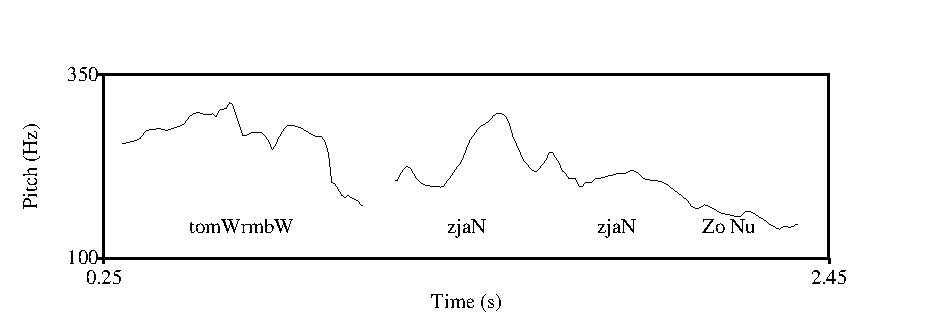
\includegraphics{sentence1.eps}
\end{figure}

 \begin{figure}
 \caption{F0 of the sentence with plain pronunciation   (sound file n°2). }
\label{fig:zjaNzjaN2}  
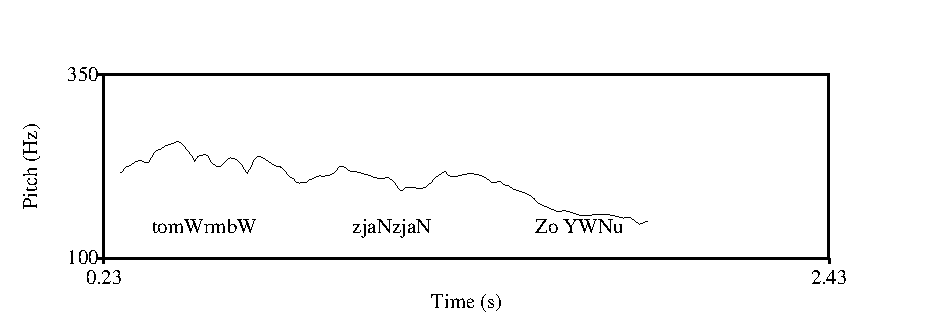
\includegraphics{sentence2.eps}
\end{figure}



Data is lacking to provide a detailed account of the   discourse function of the emphatic pronunciation of ideophones.  Only two observations can be proposed at this stage concerning the distribution of emphatic ideophones (which are   rare  in comparison with than non-emphatic ones). 

First, when the same ideophone occurs more than one time in the same narrative, the emphatic variant will be restricted to its first occurrence, as in the case in the example at hand. 

Second, highly lexicalized and conventional uses of ideophones (for instance, the colour ideophone \ipa{zɯŋzɯŋ} when applied to the hair of an old man) are not attested with emphatic pronunciation in our corpus.



  \section{Syntactic properties of ideophones}
As pointed out by \citet[660]{dingemanse12ideo}, the markedness of ideophones is not limited to their phonology, but is also manifested in their syntactic behaviour.

Ideophones nearly always occur as verb adjuncts in Japhug. They can be used with a series of light verbs or as adjuncts of any lexical verb in either nominalized or finite form. A few examples of ideophones as noun modifiers are also attested.

As an estimate of the relative frequency of each of these three constructions, in a portion of the corpus comprising 125 ideophones, 61 occurred with light verbs, 62 with lexical verbs and 2 did not have a corresponding verb.

\subsection{Light verb constructions} \label{sec:ideophone.plus.light.verb}
 
Four light verbs can be used with ideophones in Japhug: the semantically empty stative verb \ipa{pa}, the transitive speech verb \ipa{ti} `say', the manner deixis verb \ipa{stu} `do like ....' and its reflexive form \ipa{ʑɣɤ-stu} `act like ...'.   While \ipa{pa} and \ipa{ʑɣɤ-stu} are restricted to ideophonic constructions, \ipa{ti} `say'  is the most common speech verb, and takes as its P reported speech complement clauses. Likewise,  \ipa{stu} `do like ...' is often used with nouns or complement clauses expressing the manner in which a particular action takes place. Thus, Japhug data confirm the  well-known tendency of ideophones to occur in quotative or manner deixis constructions (\citet[280-8]{guldemann08quot}).



The emphatic linker \ipa{ʑo} can be inserted between the ideophone and the light verb, as in examples \ref{ex:RYJli.Zo.YWpa}, \ref{ex:rNAB.nA.rNAB} and \ref{ex:zJWG.Zo}.  

In the following examples, the light verbs are highlighted   in small capitals; ideophones are written in bold.

The verb \ipa{pa} is a stative intransitive verb etymologically related to the transitive \ipa{pa} `close, do'. It is exclusively attested as a light verb, and requires the presence of an ideophone.  It can either appear as an inflected form as in \ref{ex:RYJli.Zo.YWpa}, or as the nominalized form \ipa{kɯ-pa} as in \ref{ex:XploR.kWpa}. It is used with ideophones describing   colour, shape or spatial disposition.
 

\begin{exe}
\ex \label{ex:RYJli.Zo.YWpa}
\gll 
\ipa{ɯ-phoŋbu}  	\ipa{nɯ}  	\ipa{rcanɯ}  	\ipa{\textbf{ʁɲɟliʁɲɟli}}  	\ipa{ʑo}  	\textsc{\ipa{ɲɯ-pa} }  \\
\textsc{3sg.poss}-body \textsc{top} \textsc{top} \textsc{ideo:stat}:huge \textsc{emph} \textsc{testim}-\textsc{light.verb} \\
\glt  `Its body, it is enormous.' (lion 17)
\end{exe}
\begin{exe}
\ex \label{ex:XploR.kWpa}
\gll
\ipa{aʑo}  	\ipa{grɯβgrɯβ}  	\ipa{ɯ-ftsa}  	\ipa{nɯ}  	\ipa{tɤ-kɯ-qawɤr}  	\ipa{ma}  	\ipa{nɯ}  	\ipa{ma}  	\ipa{\textbf{χploʁploʁ}}  	\textsc{\ipa{kɯ-pa}}  	\ipa{mɯ-pɯ-mto-t-a.}  	\\
\textsc{1sg} matsutake \textsc{3sg.poss}-nephew \textsc{top} \textsc{pfv-nmlz}:S/A-open.cap apart.from \textsc{dem} apart.from \textsc{ideo:stat}:round \textsc{nmlz:S/A}-\textsc{light.verb} \textsc{neg-pfv}-see-\textsc{pst:tr-1sg} \\
\glt `The (mushroom called) the `matsutake's nephew', I have seen ones with opened caps, but never seen one in ball shape (before the cap opens).' (grɯβgrɯβtsa, 5)
\end{exe}

In both the imperfective \ipa{tu-pa} and perfective \ipa{tɤ-pa} forms, the light verb \ipa{pa} acquires the meaning of entering into the state depicted by the ideophone, as in \ref{ex:tupa.YWNu}.
\begin{exe}
\ex \label{ex:tupa.YWNu}
\gll
\ipa{ɯ-ru}  	\ipa{nɯ} \ipa{ra}  	\ipa{nɯ-rom}  	\ipa{tɕe}  	\ipa{\textbf{rʁɤβrʁɤβ}}  	\textsc{\ipa{tu-pa}}  	\ipa{ɲɯ-ŋu}  \\
\textsc{3sg.poss}-stalk \textsc{top} \textsc{pl} \textsc{pfv}-dry \textsc{lnk} \textsc{ideo:stat}:rough \textsc{ipfv}-light.verb \textsc{testim}-be \\
\glt `Once it has dried, its stalk becomes very rough.' (sɯŋgɯɟu, 21)
\end{exe}

In our text corpus, the light verb \ipa{pa} is almost exclusively attested with pattern 2 (RR) ideophones. The only example with an ideophone from a different pattern is \ref{ex:rNAB.nA.rNAB}, but it is not isolated: similar constructions  can be elicited with other pattern 3 (R\ipa{-nɤ-}R) ideophones.
\begin{exe}
\ex \label{ex:rNAB.nA.rNAB}
\gll
\ipa{tɯrme}  	\ipa{kɯ-dɯ-dɤn}  	\ipa{ʑo}  	\ipa{tu-ŋke-nɯ}  	\ipa{tɕe,}  	\ipa{nɯ}  	\ipa{ɯ-taʁ}  	\ipa{ri}  	\ipa{ɯ-rpaʁ}  	\ipa{ɕoŋtaʁ}  	\ipa{nɯ}  	\ipa{tu-nɯ-ɬoʁ}  	\ipa{tɕe,}  	\ipa{\textbf{rŋɤβnɤrŋɤβ}}  	\ipa{ʑo}  	\textsc{\ipa{pɯ-pa}}  	\ipa{ma}  	\ipa{nɯnɯ}  	\ipa{tɤ-tɕɯ}  	\ipa{kɯ-mbɯ-mbro}  	\ipa{ci}  	\ipa{pɯ-ŋu}  	\ipa{tɕe,}  	\ipa{nɯ}  	\ipa{smɤnba}  	\ipa{pɯ-ŋu.}  \\
people \textsc{nmlz:S/A-redp}-be.many \textsc{emph} \textsc{ipfv}-walk-\textsc{pl} \textsc{lnk} \textsc{dem} \textsc{3sg}-on \textsc{loc} \textsc{3sg.poss}-shoulder over \textsc{top} \textsc{ipfv:up-auto}-come.out \textsc{lnk} \textsc{ideo:dyn}:tall.and.slender \textsc{emph} \textsc{pst.ipfv-light.verb} \textsc{lnk} \textsc{dem} \textsc{indef.poss}-boy \textsc{nmlz:S/A-redp}-tall \textsc{indef} \textsc{ipfv:up}-be \textsc{lnk} \textsc{dem} doctor \textsc{ipfv:up}-be \\
\glt `As many people were walking (on the street), his shoulder was taller (than their  head), and he looked very tall and slender as he was walking. He was a very tall man, he was a doctor.'
 (Leprosy, 68)
\end{exe}

The verb \ipa{ti}   `say' is used as a light verb with  ideophones expressing sound (example \ref{ex:zJWG.Zo}) and sensations (especially itching or pain as in \ref{ex:CYWG.Zo}). Its function as a light verb for sound ideophones is paralleled by its use with onomatopoeia which are not ideophones in the proper sense (see the discussion in  section \ref{sec:non.ideophones}).

\begin{exe}
\ex \label{ex:zJWG.Zo}
\gll
 \ipa{ɯ-tʰoʁ} 	\ipa{nɯ} 	\ipa{tɕu} 	\ipa{\textbf{zɟɯɣ}} 	\ipa{ʑo} 	\textsc{\ipa{ti}} 	\ipa{ɲɯ-ŋu,} \\
\textsc{3.sg.poss}-ground \textsc{top} \textsc{loc} \textsc{ideo:semel}:heavy.object.falling.from.a.high.place \textsc{emph} \textsc{fact}:say \textsc{testim}-be \\
\glt `(The stone) made a loud noise (as it fell) on the ground.' (The demon, 76)
\end{exe}
 
\begin{exe}
\ex \label{ex:CYWG.Zo}
\gll
\ipa{tu-kɯ-ti} 	\ipa{kɯnɤ} 	\ipa{\textbf{ɕɲɯɣ}} 	\ipa{ʑo} 	\textsc{\ipa{tu-ti}} 	\ipa{tu-mŋɤm} 	\ipa{ŋu,} \\
\textsc{ipfv-genr:A}-say also \textsc{ideo:semel}:intense.pain \textsc{emph} \textsc{ipfv}-say \textsc{ipfv}-hurt \textsc{fact}:be \\
\glt `One feels intense pain even when one talks.' (ʁzɤr 35)
\end{exe}

This peculiar use of \ipa{ti} for non-auditive perception reminds one of the uses of the perception verbs  \ipa{mtsʰɤm} and \ipa{sɤŋo}. Although these verbs are generally translated as auditory perception verbs (respectively `hear' and `listen'), in fact they    can be used for almost all  non-visual sensory perception (including touch, pain, taste and also smell in the case of    \ipa{mtsʰɤm}) as in \ref{ex:zWrzWrzWr}.\footnote{Note that \ipa{zɯrzɯrzɯr}  is not an ideophone in the proper sense here, see section \ref{sec:non.ideophones}. }
 
\begin{exe}
\ex \label{ex:zWrzWrzWr}
\gll
\ipa{ɲɯ-kɯ-sɤŋo} 	\ipa{tɕe,} 	\ipa{nɯ} 	\ipa{nɯ-ɬoʁ} 	\ipa{tɕe,} 	\ipa{\textbf{zɯrzɯrzɯr}} 	\textsc{\ipa{tu-ti}} 	\ipa{qʰe} 	\ipa{tɕendɤre} 	\ipa{tɤndɤr} 	\ipa{ɲɯ-ɬoʁ} 	\ipa{ɕti.} 	\\
\textsc{ipfv-genr}:S/P-listen \textsc{lnk} \textsc{dem} \textsc{pfv}-come.out \textsc{lnk} itchy.feeling \textsc{ipfv}-say \textsc{lnk}  \textsc{lnk} pimple \textsc{ipfv}-come.out \textsc{n.pst:}be:\textsc{affirm} \\
\glt `When it appears, one has an itchy feeling, and a pimple appears.' (khɤrɯm, 4)
\end{exe}

The transitive manner deixis verb \ipa{stu} `do like ...' most commonly appears with the non-stative ideophonic patterns 3 and 4 as in \ref{ex:lhWG.nA.lhWG} and \ref{ex:rloR.nA.rloR}. It always indicate a volitive action, unlike \ipa{pa} and \ipa{ti}. Depending on the ideophone, the verb can either have a definite P (like \ipa{ɯ-ku} `his head' in example \ref{ex:rloR.nA.rloR}) or no semantic patient (as in \ref{ex:lhWG.nA.lhWG}).

\begin{exe}
\ex \label{ex:lhWG.nA.lhWG}
\gll
\ipa{ɯ-sŋɯro} 	\ipa{lu-lɤt} 	\ipa{tɕe} 	\ipa{ɬɯɣnɤɬɯɣ,} 	\ipa{\textbf{ɬɯɣnɤɬɯɣ}} 	\textsc{\ipa{tu-ste}} 	\ipa{ɲɯ-ŋu} \\
\textsc{3sg.poss}-breath \textsc{ipfv:upstream}-throw \textsc{lnk} \textsc{ideo:dyn}:breathing.movement \textsc{ideo:dyn}:breathing.movement \textsc{ipfv}-do.like[III] \textsc{testim}-be \\
\glt `When it breathes, (one can see its body) expanding and retracting with each breath.' (Frog, 3)
\end{exe}


\begin{exe}
\ex \label{ex:rloR.nA.rloR}
\gll
\ipa{ɯ-ku} 	\ipa{ra} 	\ipa{pjɯ-nɯ-χtɕi} 	\ipa{tɕe} 	\ipa{ɯ-ku} 	\ipa{ra} 	\ipa{rloʁnɤrloʁ} 	\textsc{\ipa{tu-ste}} 	\ipa{ɲɯ-ŋu.} \\
\textsc{3sg.poss}-head \textsc{pl} \textsc{ipfv-auto}-wash \textsc{lnk} \textsc{3sg.poss}-head \textsc{pl}  \textsc{ideo:dyn}:round.and.average.size \textsc{ipfv}-do.like[III] \textsc{testim}-be \\ 
\glt `When it cleans its head, it moves it with rhythm.' (Fly, 49)
\end{exe}

The intransitive verb  \ipa{ʑɣɤ-stu} `act like...' is derived from \ipa{stu} `do like ...' by adding the reflexive prefix \ipa{ʑɣɤ--} (on this prefix, see \citealt{jacques10refl}). Like \ipa{stu} and unlike \ipa{pa}, it describes a volitional activity. It is compatible with any ideophonic pattern. With pattern 2 ideophones it means `to have a look of ...' as in \ref{ex:XtshAXtshAt.Zo.tuZGAstu}.

\begin{exe}
\ex \label{ex:XtshAXtshAt.Zo.tuZGAstu}
\gll
\ipa{spɣi} 	\ipa{ɯ-ŋgɯ} 	\ipa{lu-nɯ-te} 	\ipa{ndɤre,} 	 	\ipa{rɟɤlpu} 	\ipa{tu-ɕe} 	\ipa{rcanɯ,} 	\ipa{tu-rɤjoʁβzɯr} 	\ipa{kɯ-fse} 	\ipa{rcanɯ,} 	\ipa{\textbf{χtsʰɤχtsʰɤt}} 	\ipa{ʑo} 	\textsc{\ipa{tu-ʑɣɤ-stu}} 	\ipa{tɕe} 	\ipa{ku-rɤʑi} 	\ipa{pɯ-ŋu,} 	\ipa{βdaʁmu} 	\ipa{tu-ɕe} 	\ipa{rcanɯ,} 	\ipa{pʰɤtɕʰɯχtɤr} 	\ipa{ʑo} 	\ipa{pjɯ-te} 	\ipa{tɕe,} 	\ipa{qɯqlɯ} 	\ipa{ʑo} 	\textsc{\ipa{tu-ʑɣɤ-stu} }	\ipa{tɕe} 	\ipa{ku-rɤʑi} 	\ipa{pɯ-ŋu} 	\ipa{ɲɯ-ŋu,} 	\\
attic \textsc{3sg}-inside \textsc{ipfv:upstream-auto}-put[III] \textsc{lnk} king  \textsc{ipfv:up}-go \textsc{top:emph} \textsc{ipfv}-clean.up \textsc{inf:stat}-be.like  \textsc{top:emph} \textsc{ideo:stat}:active.small \textsc{emph} \textsc{ipfv-refl}-do.like \textsc{lnk} \textsc{ipfv}-stay \textsc{pst.ipfv}-be  lady  \textsc{ipfv:up}-go \textsc{top:emph} mess \textsc{emph} \textsc{ipfv}-put[III] \textsc{lnk} \textsc{ideo:stat}:hangdog.look \textsc{emph} \textsc{ipfv-refl}-do.like \textsc{lnk} \textsc{ipfv}-stay \textsc{pst.ipfv}-be \textsc{testim}-be \\
\glt `(The king) put (the bird) in the attic. When the kind would go up there, (the bird) would clean everything up and would be lively; when the lady would go up there, it would make a mess and have a hangdog look.' (Kunbzang 302-4)
\end{exe}
% zjɤɣnɤlɤɣ ɲɯ-ʑɣɤstu
% 他在扭动,到处东瞻西望

%tɯ-jpu	nɯ	ra	khrɯŋ-khrɯŋ	ʑo	tu-ste,	tu-sɤwɯ-wum
%     \begin{exe}
%\ex \label{ex:zjAGnAzjAG}
%\gll 
  %	\ipa{rŋgɯ}  	\ipa{nɯ}  	\ipa{li}  	\ipa{ɲo-kɤtɯɣ-cɯ,}  	\ipa{tɕe}  	\ipa{zjɤɣnɤzjɤɣ}  	\ipa{pjɤ-ʑɣɤ-stu}  	\ipa{ɕti}  	\ipa{tɕe,}  \\
  	%boulder \textsc{top} gain \textsc{evd}-meet-\textsc{evd} \textsc{lnk} \textsc{ideo:dyn}:tall \textsc{evd.ipfv-refl}-do.like \textsc{n.pst:be}:\textsc{testim} \textsc{lnk}   	\\
%\glt He met again the boulder, and it was moving around, very huge. (The divination 86-87)
%\end{exe}
Two main syntactic constructions are attested with the four light verbs presented above.

First, the light verb is the main predicate of the clause, and the ideophone appears directly before it as in examples \ref{ex:XploR.kWpa}, \ref{ex:tupa.YWNu}, \ref{ex:lhWG.nA.lhWG} and \ref{ex:rloR.nA.rloR} above. 


Second, the light verb occurs either in finite   form before a lexical verb as in \ref{ex:CYWG.Zo}, \ref{ex:XtshAXtshAt.Zo.tuZGAstu}  and \ref{ex:YWqhrWt.YWcha}. The light verb and the following verb share the same TAM categories and are either in direct contact as in \ref{ex:CYWG.Zo} and \ref{ex:YWqhrWt.YWcha} or with a linker such as \ipa{tɕe} between them as in \ref{ex:XtshAXtshAt.Zo.tuZGAstu}.

\begin{exe}
\ex \label{ex:YWqhrWt.YWcha}
\gll
\ipa{tɕe} 	\ipa{\textbf{rʁɤβrʁɤβ}} 	\textsc{\ipa{ɲɯ-pa}} 	\ipa{ɲɯ-rʁom} 	\ipa{tɕe} 	\ipa{tɕe} 	\ipa{tɯtʰɯ} 	\ipa{ɯ-taʁ} 	\ipa{kɤ-kɯ-kʰrɯ} 	\ipa{nɯ} \ipa{ra} 	\ipa{ɲɯ-qʰrɯt} 	\ipa{ɲɯ-cʰa}       \\   
\textsc{lnk} \textsc{ideo:stat}:rough \textsc{testim}-light.verb \textsc{testim}-be.rough \textsc{lnk}  \textsc{lnk} pan \textsc{3sg}-on \textsc{pfv-nmlz}:S/A-dry \textsc{top} \textsc{pl} \textsc{ipfv}-scratch \textsc{testim}-can \\        
\glt  `It is very rough, and can scratch off the dry things on the pan.' (sɯŋgɯɟu, 107) 
\end{exe}





\subsection{Lexical verbs} \label{sec:ideophone.plus.lexical.verb}
Ideophones can appear as adjuncts of   lexical verbs with a compatible meaning. This construction is almost as common as the light verb construction, and there are no restrictions on the syntactic properties of ideophone-bearing verbs: stative verbs, intransitive dynamic verbs and transitive dynamic verbs can all be used with ideophone adjuncts.

Verbs like \ipa{βzu} `make' and \ipa{lɤt} `throw' which are used in many periphrastic constructions are also included in this category. In \ref{ex:CWmCWm.tuBze} for instance, the verb \ipa{βzu} `make' serves as a light verb (it is used in the same construction with several other meteorological phenomena). Although morphologically transitive (as can be seen thanks to the stem 3 alternation), it requires an overt P \ipa{qale} `wind' and an expletive (zero) A. However, in this sentence the ideophone can be removed without changing anything else. Thus, although \ipa{βzu} here does have light verb properties, they are not specific to ideophones and it cannot be put in the same class as the light verbs studied in section \ref{sec:ideophone.plus.light.verb}.

\begin{exe}
\ex \label{ex:CWmCWm.tuBze}
\gll
\ipa{tɕe}  	\ipa{qale}  	\ipa{ci}  	\ipa{\textbf{ɕɯmɕɯm}}  	\ipa{tu-βze}  \\
\textsc{lnk} wind \textsc{indef} \textsc{ideo:stat}:drizzle \textsc{ipfv}-make[III] \\
\glt `When there is a nice little wind,' (The swallow, 35)
\end{exe}

Ideophones   appear with stative verbs as in \ref{ex:YWGWrni.tsGaRtsGaR}, but are also commonly found with 
dynamic verbs, whether intransitive (\ref{ex:bAbAB.Zo.kundzoR}) or transitive  (\ref{ex:bAbAB.Zo.kundzoR}).

\begin{exe}
\ex \label{ex:YWGWrni.tsGaRtsGaR}
\gll
\ipa{ɯ-mɲaʁ}  	\ipa{wuma}  	\ipa{nɯ}  	\ipa{ɣɯ}  	\ipa{ɯ-rkɯ}  	\ipa{nɯ} \ipa{ra}  	\ipa{ɲɯ-ɣɯrni,}  	\ipa{ɲɯ-ɣɯrni}  	\ipa{\textbf{tsɣaʁtsɣaʁ}}  	\ipa{ʑo}  \\
\textsc{3sg.poss}-eye really \textsc{top} \textsc{gen} \textsc{3sg.poss}-side \textsc{top} \textsc{pl} \textsc{testim}-be.red  \textsc{testim}-be.red \textsc{ideo:stat}:brilliant.red \textsc{emph} \\
 \glt `The sides of its eye proper are red, brilliant red.'  (Crossoptilon, 52)
 \end{exe}


\begin{exe}
\ex \label{ex:bAbAB.Zo.kundzoR}
\gll
\ipa{nɯnɯ}  	\ipa{ɯ-rcʰɤβ}  	\ipa{ɕ-tu-kɯ-ŋke}  	\ipa{qʰe,}  	\ipa{tɯ-ŋga}  	\ipa{ɯ-taʁ} \ipa{ra}  	\ipa{ɯ-mat}  	\ipa{\textbf{bɤbɤβ}}  	\ipa{ʑo}  	\ipa{ku-ndzoʁ} \\
\textsc{dem} \textsc{3sg.poss}-gap \textsc{transloc-ipfv-genr:}S/P-walk \textsc{lnk} \textsc{indef.poss}-clothes \textsc{3sg}-on \textsc{pl}  \textsc{3sg.poss}-fruit \textsc{ideo:stat}:clumping.together
\textsc{emph} \textsc{ipfv-anticaus}:attach \\
\glt `When one walks among (these plants), their fruit  attaches to one's clothes in clumps.' (ɴɢorna, 164)
\end{exe}

\begin{exe}
\ex \label{ex:brWGbrWG.Zo.tutCAt}
\gll
\ipa{rtɕhɯʁjɯ}  	\ipa{ɣɯ}  	\ipa{ɯ-rme}  	\ipa{nɯ}  	\ipa{kɯ}  	\ipa{ɲɯ-kɯ-z-rɤʑa.}  	\ipa{nɯ}  	\ipa{tɯ-ɕa}  	\ipa{a-mɤ-nɯ-ɤtɯɣ}  	\ipa{ra}  	\ipa{ma}  	\ipa{tɤndɤr}  	\ipa{\textbf{brɯɣbrɯɣ}}  	\ipa{ʑo}  	\ipa{tu-tɕɤt}  	\ipa{ɲɯ-ŋu.}  \\
caterpillar \textsc{gen} \textsc{3sg.poss}-hair \textsc{top} \textsc{erg} \textsc{ipfv-genr:S/P-caus}-itch \textsc{top} \textsc{indef.poss}-flesh \textsc{irr-neg-pfv}-touch \textsc{fact}:have.to \textsc{lnk} pimple \textsc{ideo:stat}:covered.with.little.pimples \textsc{emph} \textsc{ipfv}-take.out \textsc{testim}-be \\
\glt `The caterpillar's hair itches people, it should not touch one's flesh, otherwise it will cause a lot of little pimples to appear.' (caterpillar, 85)
\end{exe}

As in light verb constructions, the ideophones can appear  before the verb (as in \ref{ex:bAbAB.Zo.kundzoR} and \ref{ex:brWGbrWG.Zo.tutCAt}). However, unlike light verbs, lexical verbs allow ideophones to appear to their right, as in \ref{ex:YWGWrni.tsGaRtsGaR} and \ref{ex:pjWXtsABnW.phoRphoR}. Postverbal ideophones are more common with lexical verbs than are preverbal ones: out of 62 examples in the portion of the corpus on which word counts were made, 48 are postverbal and only 14 preverbal. 




 \begin{exe}
\ex \label{ex:pjWXtsABnW.phoRphoR}
\gll 
\ipa{cɤndʐi}  	\ipa{pjɯ-χtsɤβ-nɯ}  	\ipa{\textbf{pʰoʁpʰoʁ}} \ipa{ʑo}\\
musk.deer.skin \textsc{ipfv}-rub-\textsc{pl} \textsc{ideo:stat}:nice.and.tight \textsc{emph}\\
\glt `They rub the musk deer skin very tightly.' (tɕakɯɣ, 8)
\end{exe}

In combination with stative verbs, ideophones only occur postverbally: in our corpus, there are no examples of a stative verb preceded by an ideophone. 

Rgyalrong languages have extremely strict verb final syntax, and ideophones are among the very few elements that can appear  postverbally without right dislocation.\footnote{Right dislocation does occur in Japhug (see \citealt[207-8]{jacques13harmonization}) and allows any adjunct, noun phrase, postpositional phrase or verb complement to occur post-verbally. However, it is rare and has a distinctive intonation not found with post-verbal ideophones.} Only a few adverbs such as \ipa{ntsɯ} `always, each time' and sentence final particles are normally allowed after the main verb. 

Moreover, unlike the sentence-final adverbs and particles, ideophones can also occur postverbally in head-internal relative clauses as in \ref{ex:phoRphoR}. This type of example is not uncommon with ideophones, but no other part of speech allows this syntactic behaviour.

  \begin{exe}
   \ex   \label{ex:phoRphoR}
 \gll [\ipa{pɣɤtɕɯ}  	\ipa{kɤ-kɯ-nɯ-rɤloʁ}  	\ipa{\textbf{pʰoʁpʰoʁ}}]  	\ipa{nɯ}  	\ipa{ɣɯ}  	\ipa{ɯ-loʁ}  	\ipa{nɯ-ŋgɯ}  	\ipa{nɯ}  	\ipa{ra,}  	\ipa{ɯʑo}  	\ipa{ɕ-tu-ndze}  \\
 bird \textsc{pfv-nmlz:S}-auto-make.a.nest \textsc{ideo:stat}:nice.and.tight \textsc{dem} \textsc{gen} \textsc{3sg.poss}-nest \textsc{3pl.poss}-inside  \textsc{top} \textsc{pl} he \textsc{cisloc-ipfv}-eat[III] \\
 \glt  `He goes into the nests of birds that have made nice nests, and eats them.' (The buzzard, 3)
   \end{exe}  
   
   In such relatives, the indefinite determiner \ipa{ci}   `a, one' can be placed either after (\ref{ex:qhjiqhji.ci}) or before (\ref{ex:ci.xtABxtAB}) the postverbal ideophone.
   
 \begin{exe}
\ex \label{ex:qhjiqhji.ci}
\gll 
\ipa{kɯ-ɤrŋi} 	\ipa{kɯ-fse} 	\ipa{\textbf{qʰjiqʰji}} 	\ipa{ci} 	\ipa{ɣɤʑu} 	\ipa{tɕe,} \\
\textsc{nmlz:S/A}-be.green \textsc{inf:stat}-be.like \textsc{ideo:stat}:dull.colour \textsc{indef} exist:\textsc{sensory} \textsc{lnk} \\
\glt `There is one which is a little green.' (grɯβgrɯβftsa, 44)
\end{exe}
 \begin{exe}
\ex \label{ex:ci.xtABxtAB}
\gll 
 	\ipa{kɯ-jpum} 	\ipa{ci} 	\ipa{\textbf{xtɤβxtɤβ}} 	\ipa{ʑo} 	\ipa{ɲɯ-ŋu} 	\\
 	\textsc{nmlz:S/A}-be.thick \textsc{indef} \textsc{ideo:stat}:thick.and.round \textsc{emph} \textsc{testim}-be    \\
\glt `(Its stalk) is  thick and round.' (grɯβgrɯβftsa, 52)
\end{exe}

While postverbal ideophones are not found in most strict SOV languages   such as Lakhota, Japanese or Korean,  they have been described in some verb final languages such as Udihe (\citealt[381-2]{nikolaeva01udihe}) where they reportedly have almost free word order.

With preverbal ideophones, the emphatic linker \ipa{ʑo} can appear optionally between the ideophone and the verb as in as in \ref{ex:bAbAB.Zo.kundzoR} and \ref{ex:brWGbrWG.Zo.tutCAt}. In the case of postverbal ideophones, two positions of \ipa{ʑo} are possible: after the ideophone as in \ref{ex:pjWXtsABnW.phoRphoR} and \ref{ex:YWwGrum.sWNsWN.Zo} or before it, and thus between the verb and the ideophone as in \ref{ex:wGrum.Zo.sWNsWN}. There is no discernible semantic difference between the two positions, as shown by the minimal pair in \ref{ex:YWwGrum.sWNsWN.Zo} and \ref{ex:wGrum.Zo.sWNsWN}.

  \begin{exe}
\ex \label{ex:YWwGrum.sWNsWN.Zo}
\gll 
 \ipa{ɯʑo}  	\ipa{ɲɯ-wɣrum}  	\ipa{\textbf{sɯŋsɯŋ}}  	\ipa{ʑo}  \\
\textsc{3sg} \textsc{testim}-be.white \textsc{ideo:stat}:white  \textsc{emph} \\
\glt `It is very white.' (zwɤrqhɤjmɤɣ, 21)
\end{exe}
 \begin{exe}
\ex \label{ex:wGrum.Zo.sWNsWN}
\gll 
\ipa{nɯnɯ}  	\ipa{ɣɯ}  	\ipa{ɯ-ru}  	\ipa{nɯ}  	\ipa{wɣrum}  	\ipa{ʑo}  	\ipa{\textbf{sɯŋsɯŋ}}  \\
\textsc{dem} \textsc{gen} \textsc{3sg.poss}-stalk \textsc{top} \textsc{fact}:be.white \textsc{emph} \textsc{ideo:stat}:white \\
\glt `Its stalk is very white.' (ɕɯrʁaʁ 98)
\end{exe}

In addition to \ipa{ʑo}, one can also use \ipa{kɯ-fse}, the infinitival  form  of the manner deixis stative verb \ipa{fse} `be like', between the verb and the ideophone as in \ref{ex:qhjiqhji.ci}.



With a verb in a negative form, the scope of  negation can be either on the action of the verb, on the ideophone or both as in (\ref{ex:mWkomdzWnW.phoRphoR}).

 \begin{exe}
\ex \label{ex:mWkomdzWnW.phoRphoR}
\gll 
 \ipa{mɯ-cʰɯ-ɤstu-nɯ} 	\ipa{mɯ-ku-omdzɯ-nɯ} 	\ipa{\textbf{pʰoʁpʰoʁ}} 	\ipa{kɯnɤ} 	\ipa{lu-nɯpʰaʁɲɤl-nɯ} 	\ipa{tɕe,} \\
\textsc{neg-ipfv}-be.straight-\textsc{pl} \textsc{neg-ipfv}-sit-\textsc{pl} \textsc{ideo:stat}:nice.and.tight
also \textsc{ipfv}-lie.down-\textsc{pl} \textsc{lnk} \\
\glt `When they do not sit straight and nice and   lie down (on the side),' (tɯ-ci paʁ, 12)
\end{exe}

%position de ci et de kɯ-fse
%tɕe kɯ-rɟɯrɲi ʑo lbjɯlbjɯɣ ŋu 
%Juniper, 8


    \subsection{Other}
   There is a residue of examples of ideophones which do not form a constituent with either a light or a lexical verb. In example \ref{ex:zJAGzJAG.ma}, the ideophone 	\ipa{zɟɤɣzɟɤɣ} `short and thick' occurs before the postposition \ipa{ma} `apart from'. Together with the preceding classifier \ipa{tɯ-rdoʁ}  `one piece', it forms a constituent within the postpositional phrase and cannot be analyzed as an adjunct of the following nominalized verb  	\ipa{kɯ-me} `which does not exist'. In this example, 	\ipa{zɟɤɣzɟɤɣ} `upright' is a postnominal modifier, with the classifier \ipa{tɯ-rdoʁ} `one piece' acting as  the head of the clause.
   
    \begin{exe}
\ex \label{ex:zJAGzJAG.ma}
\gll 
\ipa{ma} 	\ipa{nɯnɯ} 	\ipa{ɕawurambɯm} 	\ipa{tu-ti-nɯ} 	\ipa{tɕe} 	\ipa{nɯnɯ} 	 [\ipa{tɯ-rdoʁ} 	\ipa{ʑo} 	\ipa{\textbf{zɟɤɣzɟɤɣ}}] 	\ipa{ma} 	\ipa{kɯ-me} 	\ipa{ɲɯ-ŋu} 	\ipa{khi} \\
\textsc{lnk} \textsc{dem} Shwa.ba.rwa.mbum \textsc{ipfv}-say-\textsc{pl} \textsc{lnk} \textsc{dem} one-piece \textsc{emph} \textsc{ideo:stat}:short.and.thick apart.from \textsc{nmlz}:S/A-not.exist \textsc{testim}-be \textsc{hearsay} \\
\glt `People call it `Shwaba rwa'bum', it is (a  kind of deer antler) with only one (branch), short and thick.' 
 (Deer, 72-3)
\end{exe}

This is the only example in our corpus of an ideophone occurring before a postposition. It is possible to rephrase it with a light verb as in \ref{ex:zJAGzJAG}.  
    \begin{exe}
\ex \label{ex:zJAGzJAG}
\gll \ipa{\textbf{zɟɤɣzɟɤɣ}} 	\ipa{ʑo} 	\ipa{kɯ-pa} 	\ipa{tɯ-ldʑa} 	\ipa{ma} 	\ipa{me} 	\ipa{kʰi.}  \\
\textsc{ideo:stat}:short.and.thick \textsc{emph} \textsc{nmlz}:S/A-light.verb one-\textsc{cl}:long.thing apart.from \textsc{fact}:not.exist \textsc{hearsay} \\
\glt `It  has one (horn), short and thick.' (elicited)
\end{exe}

Upon rechecking  sentence \ref{ex:zJAGzJAG.ma}, speakers did not consider it to be incorrect. Yet,  it is not possible to build comparable sentences with other postpositions, in particular the ergative \ipa{kɯ}. 

The existence of a sentence like \ref{ex:zJAGzJAG.ma}  has implications for the analysis of examples such as \ref{ex:sWBsWB.tu}.
    \begin{exe}
\ex \label{ex:sWBsWB.tu}
\gll 
   \ipa{ɯ-jwaʁ} 	\ipa{nɯ} 	\ipa{ɯ-qʰu} 	\ipa{ri} 	\ipa{ɯ-rme} 	\ipa{kɯ-fse} 	\ipa{\textbf{sɯβsɯβ}} 	\ipa{tu.} \\
   \textsc{3sg.poss}-leaf \textsc{top} \textsc{3sg}-behind \textsc{loc}    \textsc{3sg.poss}-hair \textsc{nmlz}:S/A-be.like \textsc{ideo:stat}:hairy \textsc{fact}:exist    \\
\glt `On the other side of its leaves, there are hairs.' (mɤdɤmɲɤm, 44)
\end{exe}

In this sentence, the ideophone \ipa{sɯβsɯβ}  `with hair' can be analyzed as an adjunct of the verb \ipa{tu} `exist', but it could also be viewed as a postnominal modifier of 	\ipa{ɯ-rme}  `its hair'. However, in light of the rarity of unambiguous examples like \ref{ex:zJAGzJAG.ma}, it is preferable to favour the first analysis until additional data become available.
 %test: ajouter ma
 


Japhug ideophones, while they occur in positions that are specific to them (such as post-verbally), are  restricted in their syntactic uses in comparison with those of other languages. For instance, in Siwu, \citet{dingemanse14} reports more than five constructions where ideophones can be used: adverbial, complement, holophrase, adjectival and predicative. Of these five types of construction, only two have an equivalent in Japhug: adverbial and (very marginally) adjectival. 

This is however compensated  for in Japhug by the existence of a rich deideophonic verbal morphology that in studied in section \ref{sec:deideophonic}, and which allows ideophones to be used a full predicates.

\subsection{Discourse function}
  Ideophones are  non-essential to communication in that for any sentence with an ideophone, it is possible to build another sentence without an ideophone of identical truth value. The frequency of ideophones considerably varies  in discourse. It is possible to have more than ten minutes of stories, procedural texts or conversations without a single ideophone. It is equally possible to find  multiple sentences in a row each containing an ideophone or an deideophonic verb.
  
  
Ideophones convey  rich and intricate meanings in a succinct way. In traditional stories, appropriate use of ideophones greatly contributes to the vividness of the description. For instance, in  \ref{ex:ndArndAr}, the use of the ideophones \ipa{ndɤrndɤr}     `huge and imposing'	and 	\ipa{ɲcɣɤnɤɲcɣɤt} `loud and moving around' evokes  a much more expressive picture than the  translation provided here in plain language. They report, upon hearing such a sentence, imagining huge trees and flocks of birds flying around, twitting and chirping.

\begin{exe}
\ex \label{ex:ndArndAr}
 \gll 
\ipa{nɯ}  	\ipa{ra}  	\ipa{tɤ-stu-t-a}  	\ipa{tɕe,}  	\ipa{sɯŋgɯnaχtɕin}  	\ipa{ndɤrndɤr}  	\ipa{ʑo}  	\ipa{nɯ-stu-t-a,}  	\ipa{ɯ-taʁ,}  	\ipa{pɣa}  	\ipa{\textbf{ɲcɣɤnɤɲcɣɤt}}  	\ipa{ʑo}  	\ipa{ɲɯ-mbri}  	\ipa{tɕe,}  \\
\textsc{dem} \textsc{pl} \textsc{pfv}-do.like-\textsc{pst-1sg} \textsc{lnk} deep.forest \textsc{ideo:stat}:huge \textsc{emph} \textsc{pfv}-do.like-\textsc{pst-1sg} \textsc{3sg}-on birds \textsc{ideo:dyn}:loud \textsc{emph} \textsc{testim}-call \textsc{lnk} \\
\glt `I acted this way, I created a huge and deep forest on the top of whose trees birds are twitting.' (Smanmi metog koshana4, 218-9)
\end{exe}



In conversations, at least in our corpus, ideophones are much rarer than in stories or procedural texts, and data is lacking to provide a detailed description. 

  
 \section{Deideophonic verbs} \label{sec:deideophonic}
 Japhug has a very rich and productive   system of denominal prefixes deriving verbs from nouns (see \citealt{jacques12incorp, jacques14antipassive}). Some of these denominal prefixes can be used to derive verbs out of ideophones: \ipa{ɣɤ--}, \ipa{sɤ--} and \ipa{nɯ--}.
 
 The denominal prefix \ipa{ɣɤ--} derives intransitive and transitive verbs from possessed nouns. As can be seen in Table \ref{tab:denom.GA},  verbs in \ipa{ɣɤ--} have  varied semantics. We find stative verbs expressing a property linked to the base noun, intransitive dynamic verbs describing the coming into existence of the entity designated by the base noun, or  verbs  (transitive or intransitive) designating an activity linked with the base noun (\citealt[1218]{jacques12incorp}).
 
 \begin{table}[h]
 \caption{Examples of the denominal \ipa{ɣɤ--} prefix in Japhug} \label{tab:denom.GA}
\begin{tabular}{llllll}
\toprule
noun &meaning &denominal verb & meaning\\
\midrule
 \ipa{--mdzu} &thorn & \ipa{ɣɤ-mdzu} &to have thorns \\
  \ipa{tɤ-mbɣo} &deaf (n) & \ipa{ɣɤ-mbɣo} &to be deaf \\
\midrule
 \ipa{--tsrɯ} &sprout & \ipa{ɣɤ-tsrɯ} &to sprout\\
  \ipa{--kʰɯ} &smoke & \ipa{ɣɤ-kʰɯ} &to be smoked, to have smoke \\
    \midrule
  \ipa{--rʁaʁ} &hunt (n) & \ipa{ɣɤ-rʁaʁ} &to hunt (vi) \\
   \ipa{--jmŋo} &dream (n) & \ipa{ɣɤ-jmŋo} &to dream of (vt) \\ 
  \bottomrule
  \end{tabular}
 \end{table}
 
 With ideophones, \ipa{ɣɤ--} exclusively derives intransitive dynamic verbs, whose semantics correspond to patterns 3 (R-\ipa{nɤ}-R) or 4 (R-\ipa{nɤ-l}$VC_f$) ideophones. Unlike denominal derivation in \ipa{ɣɤ--} which does not appear to be productive anymore,  deideophonic verbs in \ipa{ɣɤ--} can potentially be created from any ideophone allowing dynamic semantics.
 
Ideophonic verbs in \ipa{ɣɤ--} allow two distinct derivational forms which are correlated with pattern 3 3 (R-\ipa{nɤ}-R) or  and pattern 4 (R-\ipa{nɤ-l}$VC_f$) respectively.

 The first pattern has full reduplication of the ideophonic root and the same semantics as pattern 3 ideophones. As a result  \ref{ex:YWGAzjaNzjaN} and \ref{ex:YWGAzjaNzjaN2}, for instance, are semantically equivalent. 

 		 

     \begin{exe}
\ex \label{ex:YWGAzjaNzjaN}
\gll 
 \ipa{ɲɯ-ɣɤ-zjaŋzjaŋ}  	\ipa{ʑo}  	\ipa{jɤ-ari}  \\
 \textsc{testim-deideoph:intr-ideo}:tall   \textsc{emph} \textsc{pfv}-go[II]\\
 \ex \label{ex:YWGAzjaNzjaN2}
\gll 
 \ipa{zjaŋnɤzjaŋ}  	\ipa{ʑo}  	\ipa{jɤ-ari}  \\
 \textsc{ideo:dyn}:tall   \textsc{emph} \textsc{pfv}-go[II]\\
 \glt `He went (there), very tall.' (elicited)
\end{exe}

The second pattern involves partial reduplication, where the onset of the second syllable is replaced by \ipa{l} like pattern 4 ideophones. Its semantics are also similar to pattern 4, as shown by examples  \ref{ex:YWGAYcGAlAtnW} and \ref{ex:YcGAnAlAt} derived from the root |\ipa{ɲcɣɤt}| `loud, intensely burning'. Here, both the  pattern 4 ideophone \ipa{ɲcɣɤnɤlɤt}  and the deideophonic verb  \ipa{ɲɯ-ɣɤ-ɲcɣɤlɤt-nɯ} indicate loud voices from distinct people speaking in disorderly fashion.

     \begin{exe}
\ex \label{ex:YWGAYcGAlAtnW}
\gll 
\ipa{ɕɤfɕo}  	\ipa{pɤnmawondɤn}  	\ipa{jɤ-azɣɯt}  	\ipa{rca}  	\ipa{ma}  	\ipa{kha}  	\ipa{ɲɯ-ɣɤ-ɲcɣɤlɤt-nɯ}  \\
these.days p.n. \textsc{pfv}-arrive \textsc{top} \textsc{lnk} house \textsc{testim-deideoph:int-ideo:disorder:}loud/burning-\textsc{pl}\\
\glt `Panma 'Od.ldan has returned these days, as one can hear loud voices in his house.' (Slob.dpon 298)
\end{exe}

     \begin{exe}
\ex \label{ex:YcGAnAlAt}
\gll 
\ipa{ɲcɣɤnɤlɤt}  	\ipa{ʑo}  	\ipa{pɯ-nɯ-rɤma-nɯ}  \\
\textsc{ideo:dyn:disorder}:loud/burning \textsc{emph} \textsc{pst.ipfv-auto}-work-\textsc{pl} \\
\glt `They were speaking loudly while working.' (Slob.dpon 356)
\end{exe}

With ideophonic roots designating concrete shapes such as  |\ipa{zjɤɣ}| `tall' in \ref{ex:tuGAzjAGlAG}, this derivation  implies an irregular motion   without direction.  

     \begin{exe}
\ex \label{ex:tuGAzjAGlAG}
\gll 
\ipa{rŋgɯ}  	\ipa{nɯ}  	\ipa{ɯ-zda}  	\ipa{rŋgɯ}  	\ipa{ra}  	\ipa{kɯ-fse}  	\ipa{ku-rɤʑi}  	\ipa{mɤ-kɯ-khɯ}  	\ipa{ci,}  	\ipa{tɕendɤre}  	\ipa{tu-ɣɤ-zjɤɣlɤɣ}  	\ipa{nɤ}  	\ipa{tu-ɣɤ-zjɤɣlɤɣ}  	\ipa{kɯ-ra}  	\ipa{ci}  	\ipa{pjɤ-ŋu,}  	 \\
boulder \textsc{top} \textsc{3sg.poss}-companion boulder \textsc{pl} \textsc{nmlz}:S/A-be.like \textsc{ipfv}-stay \textsc{neg-nmlz}:S/A-be.able \textsc{indef} \textsc{lnk} \textsc{ipfv-deideoph:intr-ideo:disorder}:tall \textsc{lnk} \textsc{ipfv-deideoph:intr-ideo:disorder}:tall \textsc{nmlz}:S/A-have.to \textsc{indef} \textsc{evd.ipfv}-be \\
\glt  This boulder could not stay in place like the other boulders, it was always moving around, very huge.' (The divination 23-24)
\end{exe}


Derivation with \ipa{sɤ--} instead of \ipa{ɣɤ--} creates a transitive verb with comparable semantics. As a denominal prefix, we do find some examples of \ipa{sɤ--} deriving transitive action verbs. The most interesting example with this derivation is \ipa{sɤ-kʰɯ} `to smoke out, to fill with smoke (vt)' which derives from the possessed noun \ipa{--kʰɯ} `smoke' like its intransitive counterpart \ipa{ɣɤ-kʰɯ} `to be smoked'. The intransitive \ipa{ɣɤ-kʰɯ} / transitive  \ipa{sɤ-kʰɯ} pair  is unique among denominal verbs, but formally identical to deiodeophonic verb pairs like the intransitive \ipa{ɣɤ-zjɤɣlɤɣ} `move around in disorder/in all directions (of a tall/large object)' vs the transitive \ipa{sɤ-zjɤɣlɤɣ} `shake in disorder/in all directions (a long object like a stick)'.

While with   \ipa{ɣɤ--} derivation  the characteristic described by the ideophonic root is interpreted with respect to the S of the verb, in the case of   \ipa{sɤ--} derivation it applies to the P, and implies the existence of an external agent.

As with intransitive deideophonic verbs in \ipa{ɣɤ--}, there are two possible derivations. First, \ipa{sɤ--} appears with complete reduplication and semantics identical to pattern 3 (R-\ipa{nɤ}-R) ideophones (compare \ref{ex:YWsAzjaNzjaN} with example \ref{ex:ideo3}).

     \begin{exe}
     \ex \label{ex:YWsAzjaNzjaN}
\gll
\ipa{mbro} 	\ipa{ɲɯ-sɤ-zjaŋzjaŋ} 	\ipa{ʑo} 	\ipa{ɲɯ-ɤz-nɯmbrɤpɯ} \\
horse \textsc{testim-deideoph:tr-ideo}:tall \textsc{emph} \textsc{testim-prog}-ride \\
\glt  `He looks very tall riding his horse.' (elicited)
\end{exe}

Second,  \ipa{sɤ--}  can be combined with partial reduplication in \ipa{l} implying a disorderly action as in \ref{ex:YWsAzjaNlaN}, with the same semantics as pattern 4 ideophones.

     \begin{exe}
     \ex \label{ex:YWsAzjaNlaN}
\gll
 \ipa{laʁjɯɣ}  	\ipa{ɲɯ-sɤ-zjaŋlaŋ}  \\
  staff \textsc{testim-deideoph:tr-ideo:disorder}:tall \\
  \glt `He sways the staff in all directions.' (elicited)
\end{exe}

In addition, it is possible to derive   verbs with the prefix \ipa{nɯ--} without reduplication.\footnote{On the semantics of \ipa{nɯ--} as a denominal prefix, see \citealt{jacques14antipassive}.} These (dynamic) transitive verbs express an action resulting in a state whose semantics corresponds to  pattern 2 ideophones. Thus, example \ref{ex:tanWzjaN} has the same meaning as \ref{ex:zjaNzjaN3}. 

     \begin{exe}
     \ex \label{ex:tanWzjaN}
\gll
\ipa{ɯʑo} 	\ipa{kɯ} 	\ipa{ta-nɯ-zjaŋ} 	\ipa{ʑo} 	\ipa{ta-rmbɯ} \\
he \textsc{erg} \textsc{pfv:3$\rightarrow$3'-deideoph:stative-ideo}:tall \textsc{emph} \textsc{pfv}:3$\rightarrow$3'-pile.up  \\
\glt  He piled it up very high.' (elicited)
\end{exe}

Example \ref{ex:panWCkrAG} shows the same use with a verb derived from the ideophonic root |\ipa{ɕkrɤɣ}|, which means  `lying on a hard and cold surface'.

     \begin{exe}
     \ex \label{ex:panWCkrAG}
\gll
\ipa{tɤ-aʑɯʑu-ndʑi} 	\ipa{tɕe,} 	\ipa{ɯ-zda} 	\ipa{pa-nɯ-ɕkrɤɣ} 	\ipa{ʑo} 	\ipa{pa-tʂaβ} \\
\textsc{pfv}-wrestle-\textsc{du} \textsc{lnk} \textsc{3sg.poss}-companion \textsc{pfv:3$\rightarrow$3'-deideoph:stative-ideo}:lying.on.a.hard.surface \textsc{emph} \textsc{pfv:down:3$\rightarrow$3'}-cause.to.fall.down \\
\glt `When they wrestled, he threw his adversary on the hard and cold ground.' (elicited) 
\end{exe}


Deideophonic verbs, whether transitive or intransitive, can be used as predicates in their own right as in \ref{ex:YWGAYcGAlAtnW}, \ref{ex:tuGAzjAGlAG}, \ref{ex:YWsAzjaNlaN} above, or together with a non-ideophonic verb as in \ref{ex:YWGAzjaNzjaN}. 

	In the second case, the emphatic linker \ipa{ʑo} often appears between the deideophonic verb and the other one. The two verbs    share the same person and number and often (but not always, see \ref{ex:YWGAzjaNzjaN}) the same TAM forms as in \ref{ex:panWCkrAG} and \ref{ex:tAsAdoNdoNa}.
	
	     \begin{exe}
     \ex \label{ex:tAsAdoNdoNa}
\gll
	\ipa{qʰɤjŋgɯ} 	\ipa{tɯ-ci} 	\ipa{tɤ-sɤ-doŋdoŋ-a} 	\ipa{pɯ-lat-a}\\
gutter \textsc{indef.poss}-water \textsc{pfv-deideoph:tr-ideo}:flowing.noisily-\textsc{1sg} \textsc{pfv:down}-throw-\textsc{1sg} \\
\glt `I dumped the water in the gutter (causing it to make a lot of noise).' (elicited)
\end{exe}

Just like ideophones, deideophonic verbs can appear before or after the other verb. Thus, \ref{ex:YWsAzjaNzjaN} can be rephrased as \ref{ex:YWsAzjaNzjaN2}.

     \begin{exe}
     \ex \label{ex:YWsAzjaNzjaN2}
\gll
\ipa{mbro} 		\ipa{ɲɯ-ɤz-nɯmbrɤpɯ} \ipa{ɲɯ-sɤ-zjaŋzjaŋ} 	\ipa{ʑo} \\
horse  \textsc{testim-prog}-ride \textsc{testim-deideoph:tr-ideo}:tall \textsc{emph}\\
\glt `He looks very tall riding his horse.' (elicited)
\end{exe}

With impersonal meteorological phenomena, we find in Japhug morphologically transitive verbs that do not allow any agent in the ergative. The verbs in question are either \ipa{βzu} `make' or \ipa{lɤt} `throw'. When a deideophonic verb occurs in these constructions, both the transitive \ipa{sɤ--} or the intransitive \ipa{ɣɤ--} can be used interchangeably. Thus, in \ref{ex:YWsACWmCWm}, either transitive	\ipa{ɲɯ-sɤ-ɕɯmɕɯm} or 	intransitive \ipa{ɲɯ-ɣɤ-ɕɯmɕɯm} would be possible.

     \begin{exe}
     \ex \label{ex:YWsACWmCWm}
\gll
\ipa{tɯmɯ} 	\ipa{ɲɯ-sɤ-ɕɯmɕɯm} 	\ipa{ʑo} 	\ipa{ɲɯ-ɤsɯ-lɤt} \\
sky \textsc{testim-deideoph:tr-ideo}:drizzle \textsc{emph} \textsc{testim-prog}-throw \\
\glt `It is drizzling.' (elicited)
\end{exe}
%tɯmɯ ɲɯ-sɤɕɯmɕɯm ʑo ɲɯ-ɤsɯ-lɤt
 
Some deideophonic verbs are used in idiomatic expressions whose meaning cannot be predicted. The most common such example is \ref{ex:chAnWsAYGAYcGAtnW}, which appears as the conclusion of most traditional stories and would correspond to English `They lived happily ever after'.

     \begin{exe}
\ex \label{ex:chAnWsAYGAYcGAtnW}
\gll 
\ipa{tɯ-rma}  	\ipa{tɯ-βlɯ}  	\ipa{cʰɤ-nɯ-sɤ-ɲcɣɤɲcɣɤt-nɯ}  	\ipa{kɤ-ti}  	\ipa{ɲɯ-ŋu}  \\
\textsc{nmlz:action}-live.at \textsc{nmlz:action}-burn \textsc{evd-auto-deideoph:tr}-ideo:loud/burning-\textsc{pl} \textsc{nmlz}:P-say \textsc{testim}-be \\
\glt  `They lived a prosperous and thriving (=burning) life, it is said.' (many examples)
\end{exe}

%The semantics of deideophonic verbs is not always predictable from the   ideophones themselves. For instance, the 

% tɯ-khɤl ri ku-rɤʑi tɕe,
% tɕe kɯki ɯ-ʁar ʁnɯz tu-sɤndzɯrndzɯr nɤ tu-sɤndzɯrndzɯr kɯ-fse ɲɯ-ŋu
 	  
Aside from deideophonic verbs in \ipa{ɣɤ--}, \ipa{sɤ--} and \ipa{nɯ--}, we also find isolated examples derived with the prefix \ipa{a--}. All such examples are stative verbs depicting shape or spatial distribution, and can present either complete or partial reduplication of the ideophonic  root. From instance, from the ideophonic roots |\ipa{brɤl}| `sparse and scattered (as of trees)' and |lju| `cylindrical' it is possible to derive the verbs \ipa{abrɤlbrɤl} `to be sparse' and \ipa{alɯlju} `to be cylindrical' with reduplication of the root.
 
 \section{Deideophonic nouns}
While Japhug has  deideophonic verbs, there is no corresponding regular derivation producing nouns. Yet we do find ideophonic elements in the formation of some nouns and classifiers.
 
 
 
 
 First, ideophones appear in compound nouns. The best example is \ipa{jaʁmɤzdoʁzdoʁ} `bird sp.'. The first element of this compound \ipa{jaʁmɤ--} is the \textit{status constructus} form of the possessed \ipa{--jaʁmu} `thumb', itself derived from \ipa{--jaʁ} `hand' and \ipa{--mu} `mother' (see \citealt{jacques12incorp} for more detail on vowel alternations in nominal compounds). The second element \ipa{zdoʁzdoʁ} is a pattern 2 ideophone meaning `small and active'.


Second, we find classifiers which appear to be derived from ideophones. For instance, \ipa{tɯ-boʁ} `one group (people, animals)' is clearly related to the ideophone |\ipa{boʁ}| `as a group'. Here the absence of obvious etymology, and the presence of a voiced initial \ipa{b--}, suggests that the direction of derivation is indeed from ideophone to classifier rather than the other way round.

Another such case is the classifier \ipa{tɯ-tɤxɯr} `one round, one circle (around a field for instance)', whose root is related to the ideophone |\ipa{xɯr}|  `round, rotating'. Here the derivation took place in two steps, first from  |\ipa{xɯr}|   to the unattested noun *\ipa{tɤ-xɯr} then from this noun to the classifier \ipa{tɯ-tɤxɯr}.


\section{What Ideophones are not} \label{sec:non.ideophones}
Three classes of words present common properties with, but are distinct from, real ideophones: onomatopoeia, interjections and calling sounds. Although all three also present phonological markedness and some degree of iconicity, they are not subject to ideophonic morphology as described in \ref{sec:ideo:morpho} and do not share the same syntactic properties.
 \subsection{Onomatopoeia}
While many ideophones are clearly of onomatopoeic nature, not all onomatopoeia are ideophones in Japhug. In particular, imitation of animal calls, as in \ref{ex:cutcutcut}, may not always be subject  to  ideophonic morphology as described in \ref{sec:ideo:morpho}. Besides, they are generally reduplicated three or more times and thus their forms cannot be compared with any of the nine ideophonic patterns.

     \begin{exe}
\ex \label{ex:cutcutcut}
\gll 
 	\ipa{ɲɯ-xtɕi} 	\ipa{tsa,} 	\ipa{tu-mbri} 	\ipa{nɯ} \ipa{ra} 	\ipa{cut cut cut} \ipa{ʑo} 	\ipa{tu-ti} 	\ipa{ɲɯ-ŋu;} \\
\textsc{testim}-be.small a.little \textsc{ipfv}-call \textsc{top} \textsc{pl} onomatopoiea \textsc{emph} \textsc{ipfv}-say \textsc{testim}-be \\
\glt  `It is small, and when it calls it makes `cut cut cut'.' (ʑmbrɯpɣa, 8)
\end{exe}
 
 This type of onomatopoeia has in common with   ideophones   compatibility with the light verbs \ipa{ti} `say' and \ipa{pa} `auxiliary', but has not fully entered the ideophonic morphological system and cannot serve as verb adjuncts. Onomatopoiea are commonly triplicated or even reduplicated more than three times, unlike real ideophones:  unlike languages such as Chintang (\citealt{rai06triplication}), triplication is not part of the regular ideophonic morphology.
 
 \subsection{Interjections}
 
 Interjections are marked words   expressing a feeling or an emotion   like ideophones, but unlike them, they are typically \textit{involuntary responses} to stimuli   (\citealt{dingemanse11phd}). In Japhug, they cannot serve as verb adjuncts, cannot receive ideophonic morphology and are used either in isolation, in their own clause (\ref{ex:aCi}) or as the P of verbs of speaking like \ipa{ti} `say' (\ref{ex:atsatsa}). 

       \begin{exe}
\ex \label{ex:aCi}
\gll 
\ipa{aɕi!} 	\ipa{ɲɯ-tɯ-ɣɤŋgi.} \\
\textsc{interjection}:correction \textsc{testim}-2-be.right \\
\glt `Of course (I take back what I have said) ! You are right.' (The demon, 44)
\end{exe}
      \begin{exe}
\ex \label{ex:atsatsa}
\gll 
 	\ipa{tɤ-ɣɤndʐo} 	\ipa{tɕe} 	\ipa{wutɕʰɯtɕʰɯ} 	\ipa{ma-tɯ-ti,} 	\ipa{tɤ-sɤ-ɕke} 	\ipa{tɕe} 	 	\ipa{atsatsa} 	\ipa{ma-tɯ-ti,}  \ipa{kɯ-mŋɤm} 	\ipa{tɤ-tu} 	\ipa{tɕe} 	\ipa{atsatsa} 	\ipa{ma-tɯ-ti} 	\ipa{ra} \\
 	\textsc{pfv}-be.cold \textsc{lnk} \textsc{interjection}:cold \textsc{neg:imp}-2-say \textsc{pfv-deexp}-burn \textsc{lnk} \textsc{interjection}:pain \textsc{neg:imp}-2-say \textsc{nmlz}:S/A-hurt \textsc{pfv}-exist \textsc{lnk} \textsc{interjection}:pain \textsc{neg:imp}-2-say \textsc{fact}:have.to  	\\
\glt `When you will feel cold, don't say 'Ah', when you will feel hot, don't say 'ouch', when you will feel pain, don't say 'ouch'.' (The flood3, 64)
\end{exe}
  
 Interjections in Japhug include  \ipa{wudzɯdzi} `expressing fear',  \ipa{ama} `expressing surprise', \ipa{xɯcʰɯcʰo} `expressing tiredness', \ipa{atsatsa} `expressing pain', \ipa{wutɕʰɯtɕʰɯ} `expressing cold' and \ipa{aɕi} `taking back the words one has just said'.
 
 Phonologically, these words are unusual in different ways from ideophones. They do not contain rare phonemes or clusters, but almost all start in \ipa{a--} or \ipa{wu--}. While verbs whose stem starts  in \ipa{a--} are relatively common in Japhug, the initial \ipa{a--} generally undergoes   morphonological alternations and can only surface as such in non-past forms (see \citealt{jacques07passif}).  No   single verb has a stem containing  a syllable \ipa{wu--}. Nouns whose stem starts in \ipa{a--} and \ipa{wu--}   are extremely rare. Apart from \ipa{akarɯ} `marjoram', all examples are borrowings from Tibetan (such as \ipa{araʁ} `liquor', \ipa{amɯrga} `Westerner'\footnote{This word, borrowed from English `American' through Tibetan, was translated to me into Chinese as meaning `Albanian' \zh{阿尔巴尼亚人},  a curious confusion which no doubt occurred during the cultural revolution before 1971.} or \ipa{wulaʁ} `corvée, statute labour').

\subsection{Calling  and chasing sounds}

Calling and chasing sounds are sounds used by people to interact with animals. They are used either to incite the animals to come forward in the direction of the speaker (calling sounds) or to advance (chasing sounds). In Japhug, nearly all domestic animals, whether mammals or birds, have special dedicated calling sounds, a list of which is provided in Table \ref{tab:calling.sounds}
\begin{table}[h]
\caption{Calling and chasing sounds in Japhug} \label{tab:calling.sounds}
\begin{tabular}{lllll}
\toprule
 & 	animal & 	order \\ 	
 \midrule
\ipa{tɕʰa} & 	cat & 	chasing \\ 	
\ipa{tɕítɕi tɕítɕi tɕítɕi} & 	cat & 	calling \\ 	
\ipa{wɯle} & 	cow & 	chasing \\ 	
\ipa{aβleβle} & 	cow & 	calling \\ 	
\ipa{tsaʔ tsaʔ} & 	dog & 	calling \\ 	
\ipa{soŋ} & 	dog & 	chasing \\ 	
\ipa{tʂutʂutʂutʂutʂutʂu} & 	fowl & 	calling \\ 	
\ipa{kɕɯt} & 	fowl & 	chasing \\ 	
\ipa{titititi} & 	goat & 	calling \\ 	
\ipa{kʰɯɕɯ} & 	goat, sheep & 	chasing \\ 	
\ipa{χɤj} & 	horse & 	chasing \\ 	
\ipa{a̤ a̤ a̤ a̤} & 	horse & 	calling \\ 	
\ipa{zʁozʁozʁozʁo} & 	hybrid yak (female) & 	calling \\ 	
\ipa{achocho} & 	hybrid yak (male) & 	calling \\ 	
\ipa{buwo} & 	ox & 	chasing \\ 	
\ipa{tɕʰɤt} & 	pig & 	chasing \\ 	
\ipa{anininini, ʔwan, ʔwan ʔwan} & 	pig (adult) & 	calling \\ 	
\ipa{anininini ǀǀǀǀǀǀ} & 	pig (little) & 	calling \\ 	
\ipa{alolo} & 	sheep & 	calling \\ 	
\bottomrule
\end{tabular}
\end{table}
Given the rudimentary nature of man-animal interactions, it is not surprising that these sounds cannot be subjected to any morphological  operation other than reduplication. They cannot be used with any light verbs or occur as adjuncts.


Phonologically, these words contain very unusual sounds. Unlike ideophones, which contain unusual clusters or rare phonemes, calling sounds make use of consonants and vowel that are not found at all in the standard lexicon: the dental click  \ipa{ǀ}, the glottal stop in a cluster [ʔw] or as a coda and breathy voice.

Only one of these words appears to have an identifiable etymology: \ipa{soŋ} `chasing sound for dogs' is possibly related to the past tense \ipa{soŋ} of the verb `to go' in Tibetan. 

 \section{Conclusion}
 
Japhug ideophones are an exceptionally rich topic, and the present work only scratches the surface. Future studies will have to provide as complete as possible a list of ideophones  with clear indications as to which pattern is attested for each particular ideophone and with example sentences for each of them, and investigate in more detail their uses in discourse.


Another topic for future research involves comparison with other Rgyalrong languages; preliminary work on Situ and Zbu Rgyalrong, as well as comparison with \citet{jackson04zhuangmaoci} indicate that some ideophones are shared between several varieties; the question of whether some ideophones are inherited from proto-Rgyalrong (if they present the regular sound laws) and how they are diffused across dialects will only be possible when comparable work, including comprehensive lists of ideophones, is undertaken on as many dialects as possible.
 
\bibliographystyle{linquiry2}
\bibliography{bibliogj}

 \end{document}
 